%% Verze pro jednostranný tisk:
%\documentclass[11pt,a4paper]{report}
%\usepackage[top=25mm,bottom=25mm,right=25mm,left=30mm,head=12.5mm,foot=12.5mm]{geometry}
%\let\openright=\clearpage

%% Pokud tiskneme oboustranně:
\documentclass[11pt,a4paper,twoside,openright]{report}
\usepackage[top=25mm,bottom=25mm,right=25mm,left=30mm,head=12.5mm,foot=12.5mm]{geometry}
\let\openright=\cleardoublepage

%% Definice různých užitečných maker (viz popis uvnitř souboru)
%%% Tento soubor obsahuje definice různých užitečných maker a prostředí %%%
%%% Další makra připisujte sem, ať nepřekáží v ostatních souborech.     %%%

\usepackage[a-2u]{pdfx}     % výsledné PDF bude ve standardu PDF/A-2u

%%% Nastavení pro použití samostatné bibliografické databáze.
\usepackage[
   backend=biber
%  ,style=iso-authoryear
  ,style=iso-numeric
  ,sortlocale=cs_CZ
  ,bibencoding=UTF8
  %,block=ragged
]{biblatex}
\let\cite\parencite
\bibliography{literatura}

%% Přepneme na českou sazbu, fonty Latin Modern a kódování češtiny
\usepackage[british,UKenglish,USenglish,english,american]{babel}
\usepackage{lmodern}
\usepackage[T1]{fontenc}
\usepackage{textcomp}
\usepackage[utf8]{inputenc}

%%% Další užitečné balíčky (jsou součástí běžných distribucí LaTeXu)
\usepackage{amsmath}        % rozšíření pro sazbu matematiky
\usepackage{amsfonts}       % matematické fonty
\usepackage{amsthm}         % sazba vět, definic apod.
\usepackage{bm}             % tučné symboly (příkaz \bm)
\usepackage{graphicx}       % vkládání obrázků
\usepackage{fancyvrb}       % vylepšené prostředí pro strojové písmo
\usepackage{fancyhdr}       % prostředí pohodlnější nastavení hlavy a paty stránek
\usepackage{icomma}         % inteligetní čárka v matematickém módu
\usepackage{dcolumn}        % lepší zarovnání sloupců v tabulkách
\usepackage{booktabs}       % lepší vodorovné linky v tabulkách
\usepackage{listings}
\usepackage{xcolor}
\usepackage[ruled,vlined]{algorithm2e}
\usepackage[most]{tcolorbox}
\lstdefinestyle{base}{
  language=sh,
  emptylines=1,
  breaklines=true,
  basicstyle=\small\ttfamily\color{white},
  moredelim=**[is][\color{green}]{@}{@},
}
\newtcblisting{commandshell}{colback=black,colupper=white,colframe=gray!75!black,
listing only,listing options={language=sh,style=base}}

\makeatletter
\@ifpackageloaded{xcolor}{
   \@ifpackagewith{xcolor}{usenames}{}{\PassOptionsToPackage{usenames}{xcolor}}
  }{\usepackage[usenames]{xcolor}} % barevná sazba
\makeatother
\usepackage{multicol}       % práce s více sloupci na stránce
\usepackage{caption}
\usepackage{enumitem}
\setlist[itemize]{noitemsep, topsep=0pt, partopsep=0pt}
\setlist[enumerate]{noitemsep, topsep=0pt, partopsep=0pt}
\setlist[description]{noitemsep, topsep=0pt, partopsep=0pt}

\usepackage{tocloft}
\setlength\cftparskip{0pt}
\setlength\cftbeforechapskip{1.5ex}
\setlength\cftfigindent{0pt}
\setlength\cfttabindent{0pt}
\setlength\cftbeforeloftitleskip{0pt}
\setlength\cftbeforelottitleskip{0pt}
\setlength\cftbeforetoctitleskip{0pt}
\renewcommand{\cftlottitlefont}{\Huge\bfseries\sffamily}
\renewcommand{\cftloftitlefont}{\Huge\bfseries\sffamily}
\renewcommand{\cfttoctitlefont}{\Huge\bfseries\sffamily}

% vyznaceni odstavcu
\parindent=0pt
\parskip=11pt

% zakaz vdov a sirotku - jednoradkovych pocatku ci koncu odstavcu na prechodu mezi strankami
\clubpenalty=1000
\widowpenalty=1000
\displaywidowpenalty=1000

% nastaveni radkovani
\renewcommand{\baselinestretch}{1.20}

% nastaveni pro nadpisy - tucne a bezpatkove
\usepackage{sectsty}    
\allsectionsfont{\sffamily}

% nastavení hlavy a paty stránek
\fancyhf{}
\fancyhead[RO,LE]{\rightmark}
\fancyfoot[RO,LE]{\thepage}
\renewcommand{\footrulewidth}{.5pt}
\fancypagestyle{plain}{%
\fancyhf{} % clear all header and footer fields
\fancyfoot[RO,LE]{\thepage}
\renewcommand{\headrulewidth}{0pt}
\renewcommand{\footrulewidth}{0.5pt}}

% Tato makra přesvědčují mírně ošklivým trikem LaTeX, aby hlavičky kapitol
% sázel příčetněji a nevynechával nad nimi spoustu místa. Směle ignorujte.
\makeatletter
\def\@makechapterhead#1{
  {\parindent \z@ \raggedright \sffamily
   \Huge\bfseries \thechapter. #1
   \par\nobreak
   \vskip 20\p@
}}
\def\@makeschapterhead#1{
  {\parindent \z@ \raggedright \sffamily
   \Huge\bfseries #1
   \par\nobreak
   \vskip 20\p@
}}
\makeatother

% Trochu volnější nastavení dělení slov, než je default.
\lefthyphenmin=2
\righthyphenmin=2

% Zapne černé "slimáky" na koncích řádků, které přetekly, abychom si
% jich lépe všimli.
\overfullrule=1mm

%% Balíček hyperref, kterým jdou vyrábět klikací odkazy v PDF,
%% ale hlavně ho používáme k uložení metadat do PDF (včetně obsahu).
%% Většinu nastavítek přednastaví balíček pdfx.
\hypersetup{unicode}
\hypersetup{breaklinks=true}
\hypersetup{hidelinks}

%%% Prostředí pro sazbu kódu, případně vstupu/výstupu počítačových
%%% programů. (Vyžaduje balíček fancyvrb -- fancy verbatim.)

\DefineVerbatimEnvironment{code}{Verbatim}{fontsize=\small, frame=single}


\definecolor{eclipseStrings}{RGB}{42,0.0,255}
\definecolor{eclipseKeywords}{RGB}{127,0,85}
\colorlet{numb}{magenta!60!black}

\lstdefinelanguage{json}{
    basicstyle=\normalfont\ttfamily,
    commentstyle=\color{eclipseStrings}, % style of comment
    stringstyle=\color{eclipseKeywords}, % style of strings
    numbers=left,
    numberstyle=\scriptsize,
    stepnumber=1,
    numbersep=8pt,
    showstringspaces=false,
    breaklines=true,
    frame=lines,
    string=[s]{"}{"},
    comment=[l]{:\ "},
    morecomment=[l]{:"},
    literate=
        *{0}{{{\color{numb}0}}}{1}
         {1}{{{\color{numb}1}}}{1}
         {2}{{{\color{numb}2}}}{1}
         {3}{{{\color{numb}3}}}{1}
         {4}{{{\color{numb}4}}}{1}
         {5}{{{\color{numb}5}}}{1}
         {6}{{{\color{numb}6}}}{1}
         {7}{{{\color{numb}7}}}{1}
         {8}{{{\color{numb}8}}}{1}
         {9}{{{\color{numb}9}}}{1}
}

%%% Údaje o práci
% Název práce v jazyce práce (přesně podle zadání)
\def\NazevPrace{Aspect-based sentiment analysis of conference review forms}

% Typ práce
%\def\TypPrace{BAKALÁŘSKÁ PRÁCE}
\def\TypPrace{MASTER THESIS}


% Jméno autora
\def\AutorPrace{Bc. Sára Juranková}

% Rok odevzdání. měsíc (slovně)
\def\DatumOdevzdani{December 2020}

% Vedoucí práce: Jméno a příjmení s~tituly
\def\Vedouci{prof. Ing. Vojtěch Svátek, Dr.}

% Studijní program a obor
\def\StudijniProgram{Applied Informatics}
\def\StudijniObor{Knowledge and Web Technologies}

\def\Prohlaseni{%
Prohlašuji, že jsem diplomovou práci \uv{Aspect-based sentiment analysis of
conference review forms} vypracovala samostatně za použití v práci uvedených pramenů a literatury.
}
% Nepovinné poděkování (vedoucímu práce, konzultantovi, tomu, kdo
% zapůjčil software, literaturu apod.)
\def\Podekovani{%
I would like to thank the thesis' supervisor, prof. Ing. Vojtěch Svátek, Dr., for all his guidance in writing this thesis.

I would also like to acknowledge the suffering my sister had to go through in helping me write this thesis. Few would do what she has done for me.
}

% Abstrakt (doporučený rozsah cca 150-250 slov; nejedná se o zadání práce)
\def\Abstract{%
The aim of this thesis is to create a system for extracting opinions and sentiment from conference paper reviews and group these opinions by the different criteria a paper is judged on. The theoretical part of the thesis describes the existing methods of sentiment analysis and natural language processing, thus providing necessary context. The reviewing process of conferences focused on semantic technology and the structure of the reviews are explored. A set of criteria is identified, based on the fields of different conference review forms and used as a foundation for the extraction of terms that are used to express these criteria. A sentiment lexicon is created specifically for the domain of conference paper reviews. 
In the practical section a dictionary-based sentiment lexicon analysis method is implemented and applied to a set of reviews from 3 different conferences. The results are then evaluated by comparing the numerical scores estimated by the algorithm with the numerical scores from the reviews. The outcome is then explored further, by inspecting the accuracy of criterion identification and sentiment analysis on a sentence level. The precision of criterion identification is evaluated at 57.38~\% and the recall at 53.44~\%, while the sentiment polarity is correct in  over 75~\% of cases. The rationale behind this outcome is explained and a set of recommendations is given for future improvements.

}
\def\Abstrakt{%
Cílem této práce je  vytvoření systému pro extrakci názorů a sentimentu z recenzí konferenčních příspěvků a seskupování těchto názoru podle kritérií, na základě kterých jsou tyto příspěvky posuzovány pro akceptaci.  Teoretická část práce uvádí existující metody analýzy sentimentu a zpracování přirozeného jazyka. Následně prozkoumává strukturu recenzí z konferencí zaměřených na sémantické technologie a proces, kterým tyto recenze vznikají. Na základě struktury recenzních formulářů z různých konferencí je navržena obecná množina kritérií, která jsou v této práci vytvářeným systémem z recenzních textů extrahována. Ta pak slouží jako báze k extrakci výrazů, které je vyjadřují. Rovněž je vytvořen lexikon slov se sentimentovou polaritou, specifický pro konferenční recenze. Tento lexikon je následně využit pro implementaci metody analýzy sentimentu. Ta je následně aplikována na množinu recenzí ze tří různých konferencí. Výsledky numerických odhadů pro jednotlivá kritéria jsou porovnávány s vlastním číselným hodnocením autorů recenzí. Výstup systému je dále zkoumán na úrovni vět pro zjištění správnosti identifikace kritérií a polarity sentimentu. Výsledná přesnost implementovaného algoritmu při identifikaci kritérií vychází na 57.38~\% a úplnost na 53.44~\%, přičemž  úspěšnost klasifikace sentimentu činí zhruba 75~\%. Dosažené výsledky jsou zhodnoceny a jsou navržena doporučení pro budoucí zlepšení systému.
}

% 3 až 5 klíčových slov (doporučeno)
\def\KeyWords{sentiment analysis, conference submission reviews, aspect-based sentiment analysis}
\def\KlicovaSlova{analýza sentimentu, recenze konferenčních příspěvků, aspektová analýza sentimentu}

%% Titulní strana a různé povinné informační strany
\begin{document}
%%% Titulní strana práce a další povinné informační strany

%%% Titulní strana práce

\pagestyle{empty}
\hypersetup{pageanchor=false}

\begin{center}
\Huge\sffamily
Prague University of Economics and Business\\
Faculty of Informatics and Statistics

\vspace{\stretch{1}}


\includegraphics[width=.3\textwidth]{img/logo-FIS}

\vspace{\stretch{2}}

\bfseries\NazevPrace

\vspace{8mm}
\mdseries\TypPrace

\vspace{8mm}
\large
\begin{tabular}{rl}
Study program: & \StudijniProgram \\
\noalign{\vspace{2mm}}
Field of study: & \StudijniObor \\
\end{tabular}

\vspace{\stretch{8}}

\begin{tabular}{rl}
Author: & \AutorPrace \\
\noalign{\vspace{2mm}}
Supervisor: & \Vedouci \\
\end{tabular}

\vspace{8mm}
Prague, \DatumOdevzdani
\end{center}

\hypersetup{pageanchor=true}
\cleardoublepage
\pagestyle{plain}
\openright
\vspace*{\fill}
\begin{otherlanguage}{czech}
\section*{Prohlášení}
\noindent
\Prohlaseni

\vspace*{4em}\noindent
\hfill%
\begin{tabular}[t]{c}
  5.12.2020
\end{tabular}%
\hfill%
\begin{tabular}[t]{c}
  \hbox to 12em{\leaders\hbox to 5pt{\hss . \hss}\hfil}\\ Bc. Sára Juranková
\end{tabular}%
\hfill\strut

\end{otherlanguage}
%%% Poděkování
\hypersetup{pageanchor=true}
\cleardoublepage
\pagestyle{plain}
\openright
\vspace*{\fill}
\section*{Acknowledgements}
\noindent
\Podekovani
\vspace{1cm}


%%% Povinná informační strana bakalářské práce
\openright
\section*{Abstract}
\noindent
\Abstract
\subsection*{Keywords}
\noindent
\KeyWords

\newpage
\section*{Abstrakt}
\noindent
\Abstrakt
\subsection*{Klíčová slova}
\noindent
\KlicovaSlova
\openright


%%% Strana s automaticky generovaným obsahem bakalářské práce
\setcounter{tocdepth}{2}
\tableofcontents

%%% Obrázky v bakalářské práci
\openright 
\listoffigures

%%% Tabulky v bakalářské práci (opět nemusí být nutné uvádět)
\clearpage
\listoftables

%%% Použité zkratky v bakalářské práci (opět nemusí být nutné uvádět)
\chapter*{List of Abbreviations and Acronyms}

\begin{multicols}{2}
\raggedright
\begin{description}
\item [EKAW] European Knowledge Acquisition Workshop
\item [ESWC] European Semantic Web Conference
\item [FN] False Negative
\item [FP] False Positive
\item [ISWC] International Semantic Web Conference
\item [MAE] Mean Absolute Error
\item [ML] Machine Learning
\item [NLP] Natural Language Processing
\item [NLTK] Natural Language Toolkit
\item [POS] Part Of Speech
\item [ST] Semantic Technology
\item [TP] True Positive
\end{description}
\end{multicols}



\pagestyle{fancy}
%%% Jednotlivé kapitoly práce jsou pro přehlednost uloženy v samostatných souborech
\chapter*{Introduction}
\addcontentsline{toc}{chapter}{Introduction}

The aim of this thesis is to create a system for extracting opinions and sentiment from conference paper reviews. In other words the system will allow to automatically determine the opinion of the author of the review on different aspects of the reviewed paper. 

Because each submitted paper is going to be reviewed by many people, and because each conference has its own structure of the review form as well as different set of criteria it’s very difficult to quickly get an idea of the quality of the submitted work. Being able to get a general idea of how good a paper is as well as quickly assessing what are the strong and weak parts of a submission is especially important for meta-reviewers during the discussion periods.

Extracting the opinions of the reviewer on a paper, mapping it onto a unified set of criteria and transforming it into a numerical value could significantly simplify the process of submission acceptance as well as provide a way to compare reviews of the same paper across different conferences and reviewers.

The system created here could also serve as a base for a larger review management system that is able to generate a visual metaphor of each  review that reflects different review metrics. Visual images are faster and easier to understand than written text, therefore it should make the meta-analysis more comfortable and effective.

In order to implement such a system, it’s necessary to create a set of review metrics to which the fields of different conference review forms will be mapped. Then apply a technique of information extraction to get the opinion of the reviewer on each of these metrics. In order to then get a numeric  evaluation of the sentiment of the specific opinion a sentiment analysis technique has to be used. 

%%% Fiktivní kapitola s ukázkami sazby

\chapter{Introduction to sentiment analysis and existing methods}

\section{Sentiment analysis}
Sentiment analysis (also known as opinion mining) is a type of text analysis focused on detecting polarity (e.g. positive or negative opinion) within text. This chapter serves as an introduction to the field of sentiment analysis and gives an overview of existing tools and current practices.
\subsection{Levels of sentiment analysis}
Liu \cite{liu_2015} describes 3 levels of sentiment analysis:
\begin{itemize}
    \item \textbf{Document level} -- determines the sentiment based on the entire text, which is most useful when the document expresses opinion on a single entity
    \item \textbf{Sentence level} -- classifies each sentence as positive, negative or neutral, mostly used for subjectivity classification  
    \item \textbf{Entity and Aspect level} -- recognizes the different entities described in the text and their aspects and extracts opinions linked with these aspects
    \end{itemize}
Given that the review forms express different opinions on different aspects of a paper, an opinion on a single one of these aspects can span across many sentences, sentiment analysis should therefore be done on an aspect level.
\subsection{Definition of opinion}
In order to explain the task of opinion analysis, we first need to have a definition of an opinion. This is how Liu \cite{liu_2015} defines an opinion:

\begin{quote}
An opinion is a quadruple,\begin{quote} (e, a, s, h, t)\end{quote}where $e$ is the opinion (or sentiment) target entity, $a$ is the aspect of said entity, $s$ is the sentiment about the target, $h$ is the opinion holder and $t$ is the time when the opinion was expressed. 
\end{quote}
For the needs of sentiment analysis in the task of extracting opinions from the final versions of paper reviews, a sufficient definition should be just a tuple (e, s). As reviews sometimes may have more versions than the final one, and because sometimes, a review also may contain an opinion of the author of the reviewed paper (a sentence such as "Although the author believes that his idea is novel, that is not the case" expresses the opinions of two opinion holders -- the author and the reviewer), in future the system may be improved to account for this and therefore use the original quadruple definition of an opinion.
\subsection{Classification of sentiment}

\subsection{Sentiment analysis tasks}

Another thing needing definition is the general way sentiment analysis is done.
\textcite{liu_2015} describes the task of sentiment analysis as a process of six steps, working with:
\begin{enumerate}
    \item entity extraction and categorization
    \item opinion holder extraction and categorization
    \item aspect extraction and categorization
    \item time extraction and standardization
    \item aspect sentiment classification
    \item opinion quintuple generation
\end{enumerate}

 Since conference paper review only describe one entity (the paper) and all opinions should belong to a single person (the reviewer), those parts of the analysis can be left out, as well as time extraction, since that information is not relevant in the generation of visual metaphors. Therefore the steps actually taken in the sentiment analysis of conference paper reviews are these:
 \begin{enumerate}
    \item \textbf{aspect extraction and categorization} -- Extract aspects expressions of the defined review metrics and cluster them based on the metrics they represent
    \item \textbf{aspect sentiment classification} -- Determine whether an opinion on an aspect is positive, negative or neutral and assign it a numeric value describing the polarity of the opinion as well as the strength of the sentiment
    \item \textbf{opinion tuple generation} -- produce the tuples (aspect, sentiment) based on the previous steps
    \end{enumerate}
\section{Sentiment analysis techniques}
\subsection{Machine learning}
Machine learning methods, both supervised and unsupervised, can be used for sentiment analysis. \cite{liu_2015}. For example aspect extraction can be done by Conditional Random Field (CRF), a supervised learning method commonly used in natural language processing \cite{schouten_2016}. Another technique, by Hu and Liu \cite{hu_liu_2015}, which is further explained in section \ref{Aspect Extraction} uses association mining to extract features. However most machine learning methods mostly focus on sentiment analysis on the document level.
 One such technique, which is fairly simple, but often used for simple sentiment analysis is the na\"ive Bayes classifier.
 

   \begin{figure}[htbp!]\centering
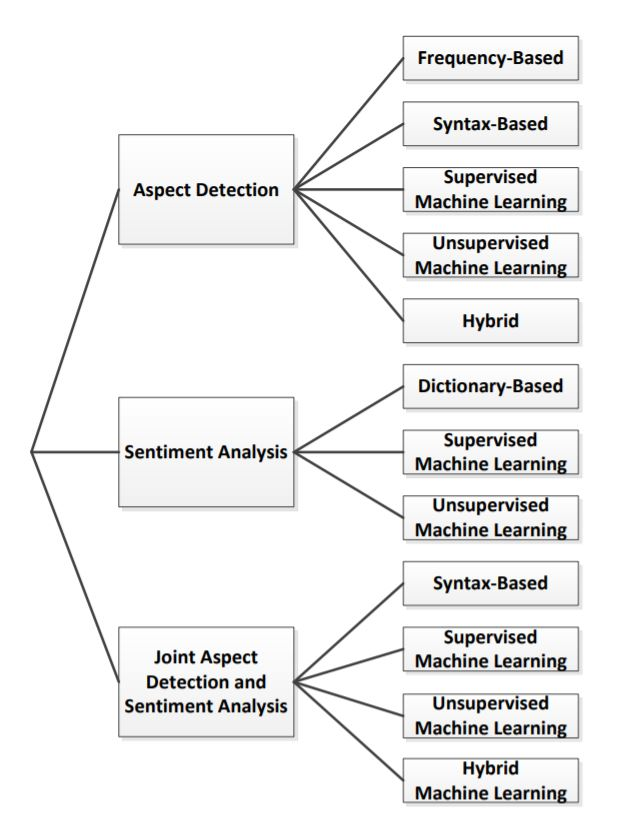
\includegraphics[width=.66\textwidth]{img/taxonomy_om}
      \caption[Taxonomy for aspect-level sentiment analysis]{Taxonomy for aspect-level sentiment analysis \cite{schouten_2016}}\label{img01:taxOM}
    \end{figure}
\subsubsection{The na\"ive Bayes classifier}
\label{sec:NBC}
 Naïve Bayes is a simple machine learning algorithm that utilizes  Bayes rule together with a strong (or na\"ive) assumption that the evidence are conditionally independent, given the hypothesis. \cite{NB}

Therefore the equation for the probability of a hypothesis $H$ given a set of evidence $E_{1},\ldots,E_{K}$, that the na\"ive Bayes classifier is based on is:

$$P\left(H|E_{1},\ldots,E_{K}\right)=\frac{P(H)}{P(E_{1},\ldots,E_{K})}\times\prod_{k=1}^{K}P\left(E_{k}|H\right)
$$

The goal of the classifier is to determine which of the possible hypothesis is the most probable given the evidence.

In the task of sentiment analysis, the different ``classes'' that serve as hypothesis are the different sentiment polarities we try to detect. So we can for example have three different classes -- positive, negative and neutral.

As I already mentioned, when classifying using the na\"ive Bayes algorithm, we look for the hypothesis for which the probability given the evidence is the highest. Therefore we can simplify the equation for $P\left(H|E_{1},\ldots,E_{K}\right)$, leaving the denominator out, because $P(E_{1},\ldots,E_{K}$ will always stay the same for all possible classes/hypothesis:

$$P\left(H|E_{1},\ldots,E_{K}\right)=P(H)\times\prod_{k=1}^{K}P\left(E_{k}|H\right)$$


The evidence are the words contained in the text we want to classify. The text is represented as a bag-of-words, meaning instead of considering the position of each word in the text, we represent it as an unordered set.

When training the na\"ive Bayes classifier we also consider the frequency of each word in each text. We also need a to have each text annotated with its sentiment. The idea behind the bag-of-word approach is depicted on figure \ref{img02:bof}
.
   \begin{figure}[htbp!]\centering
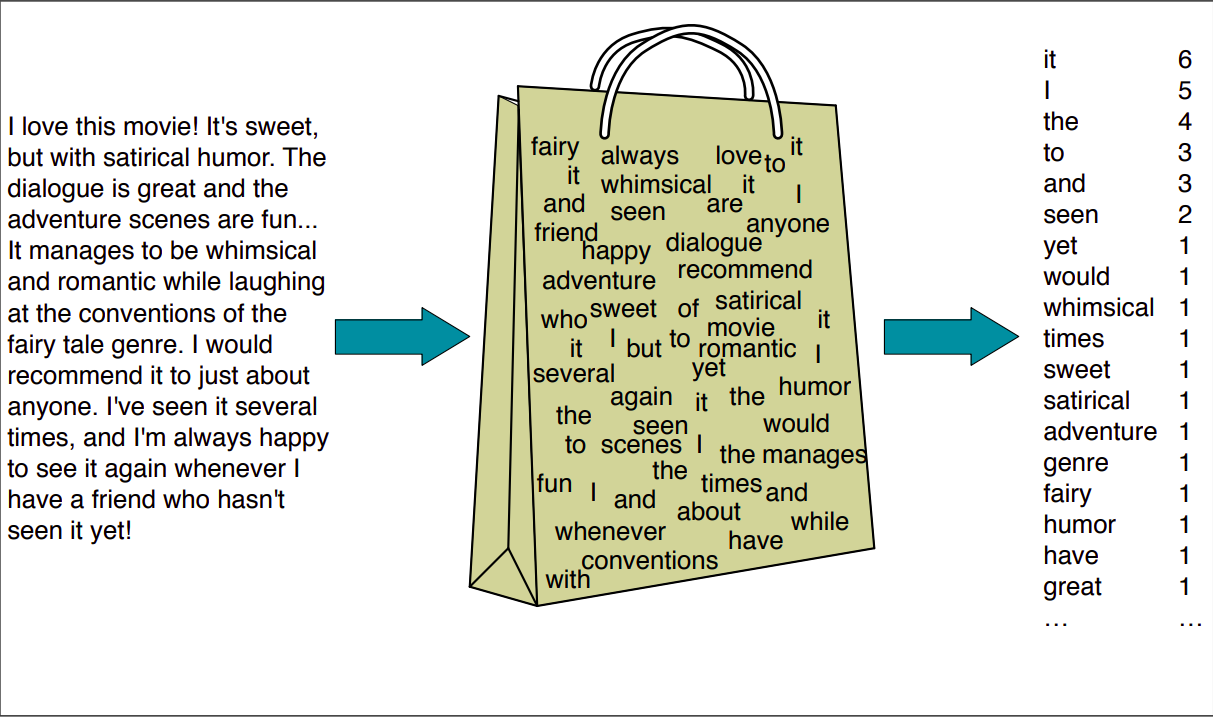
\includegraphics[width=.66\textwidth]{img/bagofwords}
      \caption[Intuition of the multinomial naive Bayes classifier applied to a movie review]{Intuition of the multinomial naive Bayes classifier applied to a movie review \cite{bagofwords}}\label{img02:bof}
    \end{figure}


Then we calculate all the necessary probabilities ($P(c)$ and $P(w_{i}|c)$ or $P(H)$ and $P(E_{k}|H)$ from the original formula) we need for classification of new texts.

The formula for the prior probability of a given class $c$ is:

$$P(c) = \frac{N_{c}}{N}$$

where $N_{c}$ is the number of text belonging to the class $c$ and $N$ is the total amount of texts in the training dataset.

The probability of a word $w_{i}$ occurring in a text with a given class $c$ is:

$$ P(w_{i}|c) = \frac{count(w_{i},c)}{\sum_{w \in V} count(w,c)} $$

where $V$ is the vocabulary, consisting of all words found across all texts, $count(w_{i},c)$ is number of times the word $w_{i}$ appears in documents belonging to class $c$ and the sum of $count(w,c)$ over all words in the vocabulary calculates the sum of all words in all documents of class $c$.

Because the na\"ive Bayes classifier multiplies all evidence likelihoods together, this equation is usually adjusted to account for the fact that some words might never appear in the training set or never appear in conjuction with some class. This makes their probability given a class zero and therefore the probability of said class also zero, independently on all the other words that appeared in the text. This behavior is usually corrected by givin these words non-zero probabilities e.g. using the add-one (Laplace) smoothing\cite{bagofwords}:

$$ P(w_{i}|c) = \frac{count(w_{i},c) + 1}{(\sum_{w \in V} count(w,c)) + |V|} $$

To give a clear example of an application of the na\"ive Bayes classifier on the task of sentiment analysis, here is how we would calculate the probability of a sentence ``This phone is great.'' being positive:

\begin{align*}
P(positive|``this",`` phone ",``is",``great")&=\\ 
&=P(``this"|positive) \\
&\times P(``phone"|positive) \\
&\times P(``is"|positive) \\
&\times P(``great"|positive)\\
&\times P(positive)
\end{align*}

\subsection{Dictionary-based Approaches}
The biggest indicators of sentiment in a text are sentiment words (also called opinion words). These words, often adjectives or adverbs, help to detect the expression of sentiment as well as its polarity. For example words such as \textit{great},\textit{amazing} or \textit{good} indicate a positive sentiment, on the other hand words like \textit{terrible}, \textit{awful} or \textit{bad} express negative feelings. \cite{liu_2015}
  
  
  In order to obtain a sentiment lexicon, Liu \cite{liu_2015} mentions 3 main approaches:
  \begin{itemize}
      \item \textbf{manual approach} -- is usually combined with automated methods because of its labor intensity
      \item \textbf{dictionary-based approach} -- usually uses a list of a small number of sentiment words as a seed and then generates the dictionary through tools such as \textcite{wordnet}   by integrating their synonyms or antonyms
      \item \textbf{corpus-based approach} -- the aim is to create a sentiment lexicon for a specific domain, for example by using a seed of sentiment words and then including other words in the lexicon by searching the sentences for conjoined adjectives, where one is already known as a sentiment word
  \end{itemize}
  There also are already compiled dictionaries of sentiment words, such as SentiWordNet \footnote{\url{https://github.com/aesuli/sentiwordnet}}, which assigns to each word both a positive score and a negative score (on a scale from 0 to 1) and allows to obtain an objectivity score based on the two. SentiWords \footnote{\url{https://hlt-nlp.fbk.eu/technologies/sentiwords}} or SenticNet \footnote{\url{https://sentic.net/}}, assign to each word they contain a sentiment score between -1 (extremely negative) and +1 (extremely positive).
  
  Lexicon-based approaches of sentiment analysis, as the name suggests, utilize lexicons of sentiment words as well as other constructs like sentiment shifters, but-clauses and other words or phrases that affect sentiment.
\subsubsection{Sentimentr}
One tool that utilizes a lexicon-based method for sentiment analysis is sentimentr.

 As explained in the sentimentr documentation ``sentimentr attempts to take into account valence shifters (i.e., negators, amplifiers (intensifiers), de-amplifiers (downtoners), and adversative conjunctions) while maintaining speed. Simply put, sentimentr is an augmented dictionary lookup.'' \cite{sentimentr}.
 
The way sentimentr works is that instead of simply comparing the words in sentence with the sentiment lexicon and judging the sentiment of a sentence based on, say, the sum of polarities of sentiment words found within it, it also adjusts the polarity of each sentiment word based on sentiment shifters found in the proximity of that word. The influence of different valence shifters is as follows:

\paragraph{Negators.} Negators are words such as ``no, not, never''. The influence of negators on the polarity of a sentiment word is simple -- if the number of negators in the left and right context of a sentiment word is even the polarity stays the same, however if the number is odd, the polarity is negated (so a word with originally negative polarity becomes positive and vice versa)

\paragraph{Amplifiers.} Amplifiers are words like ``especially, major, significantly''. As the name suggests they increase (amplify) the polarity of a sentiment word. There is however one exception to this rule -- if the number of negators in the context of a sentiment words is odd, the influence of amplifiers is negated, aka they start working as the de-amplifiers described bellow.

\paragraph{De-amplifiers} De-amplifiers, like ``slightly, somewhat sort of'' etc. work analogously to amplifiers, except they decrease the polarity of a sentiment word instead of increasing it.

\paragraph{Adversative conjuction} Adversative conjuctions are perhaps the most complex of the valence shifters. These are words such as ``bur, however, albeit''. The relative position of an adversative conjuction to the sentiment word plays an important role when determining its influence. If the conjuction comes before the sentiment word it increases its polarity, however if it comes after it decreases it. According to the sentimentr documentation ''This corresponds to the belief that an adversative conjunction makes the next clause of greater values while lowering the value placed on the prior clause.''. \cite{sentimentr}


The final sentiment score of a sentence is calculated as follows:

$$\textrm{sentiment}(s) = \frac{\sum_{w_{i} \in Pol} sentiment(w_{i})}{\sqrt{|w_{i}|}}$$

where $s$ is the sentence, $w_{i}$ is the $i$-th word of the sentence, $Pol$ is a set o polar/sentiment words in the sentence, $sentiment(w_{i})$ is the calculated sentiment of $w_{i}$ and $|w_{i}|$ is the length of the sentence.

The sentiment of a word adjusted by the valence shifters is calculated as:

\subsubsection{A Holistic Lexicon-Based Approach} 
Another lexicon-based approach is one called ``a holistic lexicon-based approach''.\cite{ding_hu_liu} This one, contrary to the \textit{sentimentr} method described above which determines the sentiment on a sentence level, focuses on aspect-based sentiment analysis. 

The basic algorithm finds all words or phrases describing features in a sentence as well as opinion (or sentiment) words. Then, for each feature in the sentence, its sentiment score is calculated using the polarity of the opinion words and their distance in the sentence from the feature expression using the following function:
$$
\textrm{score}(f) = \frac{\sum_{w_{i} : w_{i} \in s \wedge w_{i} \in V}w_{i}.SO}{dis(w_{i},f)}
$$

where:
\begin{itemize}
\item $w_{i}$ is an opinion word
\item $V$ is the set of all opinion words
\item $s$ is the sentence that contains the feature $f$
\item  $dis(w_{i} , f)$ is the distance between feature $f$ and
opinion word $w_{i}$ in the sentence $s$
\item $w i .SO$ is the semantic orientation of the word $w_{i}$
\end{itemize}
Then ``If the final score is positive, then the opinion on the feature in
the sentence s is positive. If the final score is negative, then
the opinion on the feature is negative. It is neutral otherwise.''\cite{ding_hu_liu}.

The algorithm is also extended to deal with negation (by negating the polarity of a sentiment word which follows after a negation word), ``but'' clauses (by first trying to determine the sentiment of an opinion word within the ``but'' clause using the basic algorithm and if the sentiment score is zero it assigns the negation of the clause before ``but''). Then it has these three rules for dealing with context-dependent opinion words:
\begin{itemize}
\item \textbf{Intra-sentence conjunction rule} -- this rule is based on the idea that ``a sentence only expresses one opinion
orientation unless there is a `but' word which changes the
direction.''\cite{ding_hu_liu}. Therefore if the orientation of one opinion word depends on the context but there is another opinion word in the sentence for which the orientation is known and the clauses containing the two opinion words are connected by a conjunction such as ``and'', we can assign that orientation to the context-dependent orientation word as well.
\item \textbf{Pseudo intra-sentence conjunction rule} -- this rule applies to sentences without an explicit conjunction, but otherwise works the similarly to the previous rule
\item \textbf{Inter-sentence conjunction rule} -- if the opinion orientation is still undetermined after the application of previous rules, the inter-sentence conjunction rule helps assign the orientation using the context of the surrounding sentences. According to the authors ``The idea is that people usually express the same
opinion (positive or negative) across sentences unless there is
an indication of opinion change using words such as `but' and
`however'.''\cite{ding_hu_liu}.
\end{itemize}
\section{Aspect extraction}
\subsection{Frequency extraction}
In order to extract aspect expressions, Hu and Liu \cite{hu_liu_2015} propose using a Part Of Speech (POS) tagger to identify nouns and noun phrases as possible aspect expression candidates. Then they use a simplified Apriori algorithm to calculate frequency of these candidates and finally keep only the ones that are frequent enough. 
  
  Their reasoning is that the vocabulary people use when commenting on an entity converges, so the frequently co-occurring sets of terms should represent the important aspects.
\subsection{Taxonomy based extraction}
\label{sec:taxonomy}
 Another approach, by Carenini\cite{carenini_2005}, uses user's prior knowledge of the domain to build a hierarchy of features. Their technique uses the previously mentioned unsupervised learning technique developed by Hu and Liu and adds user-defined features and similarity matching in order to eliminate redundancy  and to generate a set of features in an organized way, reflecting hierarchical relationships between them.
The way their method works is that first a set of ``crude features'' is generated by Hu and Liu's method.

Then  the WordNet lexical database is used to perform similarity matching between the user-defined taxonomy of features and the crude features. Only the crude features that are similar enough to the features already included in the taxonomy are then further used. 

Finally the newly discovered feature candidates which passed the similarity matching are inspected by a user and if the user considers these candidates valid feature expression, they are added to the final taxonomy.
\subsection{Patterns for aspect extraction}
A very different technique for aspect extraction is described by Asghar et al.\cite{asghar_2019}. Their opinion mining framework comprises of a set of heuristic patterns for extraction of aspects as well as sentiments or opinions. 

In order to get the pairs of aspects and the related sentiments, the reviews first go through a preprocessing phase, part of which is POS tagging. After that, the POS tagged sentences are matched against a set of patterns. Each pattern is a sequence of POS tags, so in order to get a match against one of them, the sentence must contain that sequence of tags as well. 

The part of the pattern which is a noun, noun phrase or a verb is then considered to be a candidate term for an aspect while mostly adjectives and adverbs represent the expression of sentiment.

\chapter{Natural language processing}
Natural language is any language that has not been artificially constructed but rather has evolved naturally through use and is  \textit{``acquired by its users without special instructions as a normal part of the process of maturization and socialization''}. \cite[p. 29]{lyons_1991}. These languages such as English, Arabic, Vietnamese or Hindi differ from non-natural languages, which are constructed for specific uses, like for example programming languages or symbolic languages used for studying logic.

Natural language processing (NLP) is \textit{``an interdisciplinary domain which is concerned with understanding natural languages as well as using them to enable human–computer interaction''} \cite[p. 1]{nlp_definition}. The field of applications of NLP is far reaching and includes use cases such as:
\begin{itemize}
\item Identifying spam e-mails \cite{nlp_tasks}
\item Chatbots for customer support and engagement \cite{nlp_uc_b}
\item Improvement in clinical documentation \cite{nlp_uc_h}	
\end{itemize}
and many others. An overview of the usage of NLP can be seen in Table \ref{tab01:nlp_tasks}.

\begin{table}[htbp!]
\caption[NLP tasks]{Breakdown of various NLP tasks performed by modern NLP software \cite{nlp_uc_b}}\label{tab01:nlp_tasks}
\small
\begin{tabular}{|l|l|l|l|}
\hline
\textbf{Word Tagging}                                               & \textbf{Sentence Parsing} & \textbf{Text Classification} & \textbf{Text Generation} \\ \hline
Word segmentation                                                   & Constituency parsing      & Sentiment analysis           & Language modeling        \\ \hline
Shallow syntax-chunking                                             & Semantic parsing          & Text classification          & Machine translation      \\ \hline
Named entity recognition                                            & Dependency parsing        & Temporal processing          & Simplification           \\ \hline
Part-of-speech tagging                                              & -                         & Coreference resolution       & Summarization            \\ \hline
Semantic role labeling                                              & -                         & -                            & Dialogue                 \\ \hline
\begin{tabular}[c]{@{}l@{}}Word sense\\ disambiguation\end{tabular} & -                         & -                            & Question answering       \\ \hline
\end{tabular}
\end{table}

It is also a very hard task, given the fact that natural languages do not adhere to the strict rules non-natural languages usually do. 
\begin{aquote}{\cite[p. 1]{nlp_lang_rules}}
\textit{``Human language is highly ambiguous\ldots It is also ever changing and evolving. People are great at producing language and understanding language, and are capable of expressing, perceiving, and interpreting very elaborate and nuanced meanings. At the same time, while we humans are great users of language, we are also very poor at formally understanding and describing the rules that govern language.''}
\end{aquote}

In fact, the \textit{imitation game}, a test developed by Alan Turing in the 50's as a test of artificial intelligence, relies on the ability of a computer program to impersonate a human in a written conversation. \cite{turing}


Because of its potential, NLP has been studied for decades (the first proposals for machine-translation pre-date the invention of the digital computer \cite{nlp_history}). 

This chapter serves as an introduction to the field of natural language processing, first describing the common tasks of NLP and then introducing some frequently used tools and methods.
\section{Common tasks in natural language preprocessing}
With many machine learning and data mining tasks, we work with data in a form of a large table, where each row represents one object and each column represents property of the objects. Most ML methods are therefore designed to work with these tables. 

When it comes to texts in natural language, they are in their raw form just a series of characters. In order to add some structure to this unstructured data, we usually perform a number of preprocessing steps, which allow us to transform the text into a representation better suited to our needs. This section focuses on the most common preprocessing steps of natural language processing.

\subsection{Tokenization}
The goal of tokenization is to separate the text into smaller units and it is \textit{``a fundamental step in both traditional NLP methods\ldots and advanced deep learning-based architectures''} \cite{tokenization}.
The text may be segmented into paragraphs, but most commonly tokenization refers to splitting the text into sentences and words. 
Tokenization can remove punctuation too, but that may cause issues such as wrongly splitting up abbreviations with periods (e.g., dr.), where the period following that abbreviation should be considered as part of the same token and not be removed. \cite{nlp_tasks}

There are different techniques of tokenization, their usage depends on the language and the purpose of tokenization, so this section provides examples of some commonly used tokenizers.
\subsubsection{White space tokenization}
White space tokenization splits the text into tokens based on white spaces, such as tabulation characters, spaces, newline characters etc.

Although this is a fast and easy way to implement tokenization, this technique only works in languages where meaningful units are separated by spaces e.g.  English, but even then, it does not work well for open compound words such as \textit{living room} or \textit{full moon}. \cite{tokenization_mgl}
\subsubsection{Dictionary based tokenization}
Dictionary based tokenization uses a dictionary of tokens to segment the text. If the token is not found in the dictionary, special rules are applied to tokenize it. \cite{tokenization_twd}

For languages without spaces between words, there is an additional step of word segmentation where we find sequences of characters that have a certain meaning. \cite{tokenization_mgl}
\subsubsection{Regular expression tokenization}
Regular expression tokenizers are rule based tokenizers, which use regular expressions to control the tokenization of text into tokens. \cite{tokenization_twd}
It is a useful technique when you want more control over the tokenization of the text by creating your own regular expression by which the text is tokenized.
\subsection{Stop words removal}
Some words, which often appear in analyzed documents, have little informational value and can be excluded. This process is called stop words removal. Stop words removal includes getting rid of common language articles, pronouns and prepositions such as \textit{and}, \textit{the} or \textit{to} in English and other words that may be considered insignificant. \cite{nlp_tasks}

Generally, the more often a word or a term appears in a collection of documents, the lesser informational value it has. Therefore the strategy for creating a list of stop words is to sort the terms by the total number of times each term appears in the document collection and pick the most frequent terms as stop words. \cite{stopwords}

Stop words removal is an especially important step in the field of information retrieval, where excluding words with little informational value tends to have a huge impact on the speed of these systems as well as the volume of data that has to be stored.
\subsection{Part-of-speech tagging}
\label{sec:pos}
Part-of-speech tagging (POS) is the process of assigning part-of-speech tags to words in a sentence. A POS tag is a label assigned to each token in a document to indicate the part of speech  and often also other grammatical categories such as tense or number (plural/singular). \cite{pos}

Because POS taggers usually tend to take into account different grammatical categories, their tag set tends to be larger that the number of part-of-speech categories of the language they are intended for. In English, there are frequently listed and thought eight parts of speech (noun, pronoun, verb, adjective, adverb, preposition, conjunction, article and interjection), but the commonly used Penn Treebank tagset contains 36 POS tags and 12 other tags (for punctuation and currency symbols). \cite{penn_treebank}
\subsection{Lemmatization and stemming}
Since documents use different forms of a word, we often need to reduce the inflectional forms and sometimes the derivationally related forms of a word to a common base form. This is especially important (and difficult) with synthetic languages which can be defined as \textit{``any language in which syntactic relations within sentences are expressed by inflection (the change in the form of a word that indicates distinctions of tense, person, gender, number, mood, voice, and case) or by agglutination (word formation by means of morpheme, or word unit, clustering). Latin is an example of an inflected language; Hungarian and Finnish are examples of agglutinative languages.''} \cite{synthetic_lang}.

The two techniques of text normalization are stemming and lemmatization.
\subsubsection{Stemming}
The algorithms knows as stemmers produce \textit{stems} of a word by cutting off the beginning and the end of the word, usually by using a list of common prefixes and suffixes. \cite{stemming_vs_lemmatization}

It is a crude heuristic process, which is why the produced stems often do not correspond to the morphological root of the word.  If given the token \textit{saw}, stemming might return \textit{saw} (or possibly just \textit{s}, whereas lemmatization (described in the next section) would likely return either \textit{see} or \textit{saw} depending on whether the use of the token was as a verb or a noun. \cite{stemming_vs_lemmatization_twd}

\subsubsection{Lemmatization}
Lemmatization is a process of applying morphological analysis to words in order to remove inflectional endings and transform the words into their base or dictionary forms called \textit{lemmas}. Lemmas unlike stems are actual language words. \cite{stopwords} 

In lemmatization the normalization depends on the part of speech of a word so it either has the be automatically determined in the previous step or this context has to be supplied in another way. 
Lemmatization is more sophisticated than stemming, producing more accurate results and meaningful tokens by considering the context, however it has is trade-offs. Compared to stemming, the process of lemmatization is slower and significantly harder to implement.

\section{Selected (Python-based) NLP tools}
As Python is \textit{``the leading coding language for NLP because of its simple syntax, structure, and rich text processing tool''} \cite{python_best} it has been chosen as the programming language for the implementation of the aspect-based sentiment analysis. This section provides a brief introduction to two of Python's NLP libraries -- NLTK and spaCy.
\subsection{Python's NLTK library}
Python's Natural Language Toolkit (NLTK) is an open source library which contains a wide range of tools and algorithms for building programs aimed at natural language processing. It provides a way to perform standard NLP tasks such as part-of-speech tagging, syntactic parsing or text classification. An overview of some NLTK modules with their functionalities is depicted in Table \ref{tab:nltk_modules}.

\begin{table}[!htb]
\caption[NLTK modules]{Language processing tasks and corresponding NLTK modules with examples of
functionality \cite{nltk_ps}}\label{tab:nltk_modules}

\begin{tabular}{lll}
\textbf{Language processing task} & \textbf{NLTK modules}                                                  & \textbf{Functionality}                                                                                     \\ \hline
Accessing corpora                 & nltk.corpus                                                            & \begin{tabular}[c]{@{}l@{}}Standardized interfaces \\ to corpora and lexicons\end{tabular}                 \\
String processing                 & \begin{tabular}[c]{@{}l@{}}nltk.tokenize, \\ nltk.stem\end{tabular}    & \begin{tabular}[c]{@{}l@{}}Tokenizers, \\ sentence tokenizers,\\ stemmers\end{tabular}                     \\
Part-of-speech tagging            & nltk.tag                                                               & \begin{tabular}[c]{@{}l@{}}n-gram, backoff, Brill, \\ HMM, TnT\end{tabular}                                \\
Classification                    & \begin{tabular}[c]{@{}l@{}}nltk.classify, \\ nltk.cluster\end{tabular} & \begin{tabular}[c]{@{}l@{}}Decision tree, \\ maximum entropy, \\ naive Bayes, k-means\end{tabular}         \\
Chunking                          & nltk.chunk                                                             & \begin{tabular}[c]{@{}l@{}}Regular expression, \\ n-gram, named entity\end{tabular}                        \\
Parsing                           & nltk.parse                                                             & \begin{tabular}[c]{@{}l@{}}Chart, feature-based, \\ unification, probabilistic, \\ dependency\end{tabular} \\
Evaluation metrics                & nltk.metrics                                                           & \begin{tabular}[c]{@{}l@{}}Precision, recall, \\ agreement coefficients\end{tabular}                       \\
Applications                      & nltk.app, nltk.chat                                                    & \begin{tabular}[c]{@{}l@{}}Graphical concordancer, \\ parsers, WordNet browser, \\ chatbots\end{tabular}  
\end{tabular}
\end{table}
\subsubsection{WordNet interface}
NLTK also provides an interface to WordNet, which is a semantically oriented dictionary of English consisting of 155289 words and 117659 synonym sets \cite{wordnet_counts}.

The WordNet interface allow us to find a list synonyms to a given word, which in the context of WordNet is called a \textit{synset}. In order to get a synset  the \texttt{synsets()} function needs to be called with the word for which the synsets are wanted as an argument along with an optional part-of-speech tag:

\begin{lstlisting}
	from nltk.corpus import wordnet
	syns = wordnet.synsets("dog")
	print(syns)
\end{lstlisting}

The function outputs a list of synsets:

\begin{lstlisting}
	[Synset('dog.n.01'), Synset('frump.n.01'),
	 Synset('dog.n.03'), Synset('cad.n.01'),
	 Synset('frank.n.02'), Synset('pawl.n.01'),
	 Synset('andiron.n.01'), Synset('chase.v.01')]
\end{lstlisting}

Each synset is identified with a 3-part name in the form <lemma>.<pos>.<number>, where:
\begin{itemize}
\item \textbf{<lemma>} is the lemma of the word
\item \textbf{<pos>} is a part-of-speech tag
\item \textbf{<number>} is the sense number used to disambiguate word meanings \cite{nltk_docs}
\end{itemize}

The interface also implements a number of ways how to find similarity between two synsets. Here are some examples along with their description taken from the WordNet interface howto guide \cite{wordnet_howto}: 

\begin{itemize}
\item \texttt{path\_similarity} returns a score denoting how similar two word senses are, based on the shortest path that connects the senses in the is-a (hypernym/hyponym) taxonomy.

\item \texttt{lch\_similarity} returns a score denoting how similar two word senses are, based on the shortest path that connects the senses (as above) and the maximum depth of the taxonomy in which the senses occur.

\item \texttt{wup\_similarity} returns a score denoting how similar two word senses are, based on the depth of the two senses in the taxonomy and that of their Least Common Subsumer (most specific ancestor node). 
\end{itemize}

Another function WordNet offers is the \texttt{derivationally\_related\_forms()} function which allows us to find terms which are in a different syntactic category but have the same root form and are semantically related to a word we supply as an argument.

\subsection{spaCy}
spaCy is NLP library for Python and Cython (a programming language written mostly in Python with additional C-inspired syntax). It is a newer library than NLTK, using an object-oriented approach as opposed to NLTK's string approach. Unlike NLTK  it has support for word vectors (multi-dimensional meaning representations of a word) and its processing is generally faster than that of NLTK (due to its Cython implementation). 
Same as NLTK it provides tools for many NLP tasks such as POS tagging, tokenization, measuring similarity between words etc. \cite{spacy}
\chapter{Description of the domain of analyzed conference paper reviews}
The data on which the analysis will be done are all from events and conferences focused on semantic technology (ST). Sentiment analysis is usually applied to product reviews or posts on social media, therefore this work will serve as an exploration of the possibility of creating a  model which, even though focused on one domain, is generalized  across various events of the same umbrella subject.

Eventually, the model can be extended to be less domain-specific, given that the review metrics probably will not differ significantly between different research areas (or at least not if we stay in the field of technology related conferences). 

In this chapter a brief introduction is given into the studied domain of conferences with focus on semantic technology and the general reviewing process a submission goes through. It is also focused on existing research on the topic of conference paper reviews.

\section{Studied conferences within the field of semantic technology}
This section serves as a description of the conferences from which the reviews studied in this work came from, which are generally focused on the topics of semantic technology and knowledge engineering.
\subsection{European Semantic Web Conference ESWC}
The European Semantic Web Conference (ESWC) is an international conference on the topic of ST which first began in 2004.
According to the ESWC website, \textit{``the mission of the ESWC is to bring together researchers and practitioners in all these areas dealing with different aspects of semantics on the Web.''} \cite{eswc}.

The topics of ESWC conferences include linked open data, machine learning, natural language processing and information retrieval, ontologies, reasoning, semantic data management, services, processes, and cloud computing, social Web and Web science, in-use and industrial, digital libraries and cultural heritage, and e-government. \cite{eswc_topics}
\subsection{European Knowledge Acquisition Workshop EKAW}
The European Knowledge Acquisition Workshop (EKAW) started in 1987 as a workshop in the field of knowledge-based systems and became a conference in 2000 changing its full title to the International Conference on Knowledge Engineering and Knowledge Management. \cite{ekaw}

As they state on their website about the 2020 EKAW conference \textit{``the 22nd International Conference on Knowledge Engineering and Knowledge Management is concerned with all aspects about eliciting, acquiring, modeling and managing knowledge, and the construction of knowledge-intensive systems and services for the semantic web, knowledge management, e-business, natural language processing, intelligent information integration, and so on''} \cite{ekaw_2020}.
\subsection{International Semantic Web Conference ISWC}
The International Semantic Web Conference (ISWC) focuses on research regarding semantic web topics including linked data. It is a successor of the Semantic Web Working Symposium (SWWS) and is held annually since 2002. \cite{iswc}


\section{Reviewing process of conference submissions}
The aim of this section is to give an overview of the steps of a reviewing process, to give the reader a better understanding on the context in which the reviews analyzed in this work are created.
While the reviewing process of different conferences may vary, there is set of general steps which they all follow to a certain degree.\footnote{Information and insights in this section are partly based on public information on the websites of the conferences and partly on private communication with the thesis’ supervisor, who has insider experience with the processes of these conferences.}

Each paper submitted to a conference is reviewed by multiple reviewers (usually three or more). After the reviewers submit their reviews authors may be able to react during a rebuttal phase, by clearing up any misunderstandings, answering questions posed by the reviewers and by defending their position on things a reviewer may have complained about. This is a common reviewing step in bigger conferences such as ISWC or ESWC however that may not be the case for smaller conferences such as EKAW where the authors only get the final reviews and whether the submission was accepted or not. Sometimes the authors get the numerical scores given by the reviewers as well as the written reviews with reviewer's comments, but occasionally only the comments are supplied so as the authors cannot use the numerical scores to argue (for example when the scores given by one reviewer are significantly higher that the scores of other reviewers).

Certain conferences also have an ``offline'' discussion amongst the reviewers, which is not accessible by the authors, usually moderated by a track chair.

Based on the reaction of the authors of the papers to the initial reviews the reviewers have the opportunity to adjust their reviews (or they should at least make it clear that they have read the author's response).

The track chair also can write meta reviews, which serve as summaries of the more in-depth reviews by the other reviewers. That is a standard step in conferences where there is also a conference chair above the track chair who makes the final decision about a paper acceptance. In that case the conference chair mostly decides based on the conclusion given in the meta review, it is quite rare for them to decide otherwise.

In terms of anonymity in the reviewing process, there are many different options and situations.  Usually the author is not given the names of reviewers, but reviewers can see the names of the authors. Occasionally conferences follow a double-blind model, where the paper's authorship is anonymized. However, that is not always possible, for example resource tracks (tracks aimed at sharing resources including datasets, software frameworks, ontologies, methodologies or metrics) are just about impossible to anonymize due to the fact that the resources the papers refer to need to be publicly available and in use. 
Sometimes conferences however do allow the authors to know the names of the reviewers (albeit the reviewers usually have the option to stay anonymous if they wish).

Certain conferences also keep the reviewers anonymous from one another or from the meta-reviewer. The goal here is to give less experienced reviewers a chance to express themselves without worrying about the opinion of senior reviewers and vice versa to keep more experienced reviewers from undermining the opinions given by a less experienced reviewer.
\section{The structure of conference paper reviews}
\label{sec:rev_structure}
Different conferences structure their reviews differently. Some are in the form of a completely unstructured text, while some clearly separate the comments in the reviews by the criteria. 

For example, the structure of the 2018 EKAW conference reviews is that there is a set of criteria which are assigned numeric scores (relevance, overall evaluation and reviewer's confidence) followed by two yes or no scoring (best paper candidate and poster \& demo candidate). It is then followed by a summary of the reviewed paper. The reviewers comments are divided into three parts: \textit{Reasons to accept}, \textit{Reasons to reject} and \textit{Overall evaluation}. The reviews also sometimes contain confidential remarks for the program committee.

The 2017 ISWC and 2018 ISWC conferences were more detailed with its numerical scoring, assigning these scores to:
\begin{itemize}
\item Reviewer's confidence
\item Appropriateness
\item Clarity and quality of writing
\item Related work
\item Originality/innovativeness
\item Impact of ideas and results
\item Implementation and soundness
\item Evaluation
\item Overall paper evaluation
\end{itemize}

Following these numerical scores, the rest of the ISWC reviews are in the form of unstructured text, unless the author of the review specifically made the decision to structure their comments either by the judged aspect or by the positivity or negativity of their comments.

The most structured reviews available to study were from the 2018 ESWC conference. There, numeric score were assigned to:
\begin{itemize}
\item Relevance to ESWC
\item Novelty of the proposed solution
\item Correctness and completeness of the proposed solution
\item Evaluation of the state-of-the-art
\item Demonstration and discussion of the properties of the proposed approach
\item Reproducibility and generality of the experimental study
\item Overall score
\end{itemize}

while the textual part of the review was clearly divided into the same categories.
\section{Previous research on conference paper reviews}
While there is quite a lot of existing research regarding information extraction from research papers, mostly used for paper summarization and extraction of keywords, not much research was found that focused on information extraction or opinion mining from the reviews of such papers.

 
In terms of possible generic metrics, previous research on this topic was done as part of a paper on the possibility of pictorial representation of review scores \cite{svatek_strossa}. The metrics they propose are these:
\begin{itemize}
    \item Relevance
    \item Novelty
    \item Technical quality
    \item State of the art
    \item Evaluation
    \item Significance
    \item Presentation
\end{itemize}
The overview of different metrics of nine conferences with focus on semantic technology and knowledge engineering and their mapping onto a set of generic criteria can be found in Table \ref{table:conf}.
\begin{landscape}
\begin{table}[p]
\caption[Mapping between generic review metrics and form fields]{Proposed mapping between generic review metrics and form fields of KE conferences \cite{svatek_strossa}}
\label{table:conf}
\small
\centering

\setlength{\defaultaddspace}{.33333\defaultaddspace}
\begin{tabular}
    {   
        L{15mm} | % gencat 
        L{18mm}  % ecai
        L{12mm}  % ekaw   
        L{60mm}  % eswc
        L{20mm}  % fois
        L{18mm}  % ijcai
        L{25mm}  % iswc
        L{16mm}  % kr     
    }
     \toprule
Review metric	&	ECAI (2016)	&	EKAW (2020)	&	ESWC (2018)	&	FOIS (2016)	&	IJCAI (2019) &	ISWC, SEMANTiCS (2018)	&	KR (2014)	\\
     \toprule
Relevance	&	Relevance	&	NA	&	Relevance to ESWC	&	NA	&	Relevance	&	Appropriateness	&	Relevance of the paper to KR	\\
\midrule
Novelty	&	Originality	&	Novelty	&	Novelty of the proposed solution	&	Novelty or innovation	&	Originality	&	Originality / innovativeness	&	Novelty of the contribution	\\
\midrule
Technical quality	&	Technical quality &	Technical soundness and depth &	Correctness and completeness of the proposed solution; Demonstration and discussion of the properties of the proposed approach	&	Scientific or technical quality	&	Technical quality	& Implementation and soundness	&	Technical quality	\\
\midrule
State of the art	&	Scholarship	&	NA	&	Evaluation of the state-of-the-art	&	References	&	Scholarship	&	Related work	&		Discussion of related work	\\
\midrule
Evaluation	&	NA	&	NA	&	Reproducibility and generality of the experimental study	&	NA	&	NA	&	Evaluation	&	NA	\\
\midrule
Significance	&	Significance	&	NA	&	NA	&	NA	&	Significance	&	Impact of ideas and results	&	NA	\\
\midrule
Presentation	&	Presentation quality	&	Clarity and quality of writing	&	NA	&	Presentation &	Clarity and quality of writing	&	Clarity and quality of writing	&		Quality of the presentation	\\
     \bottomrule
\end{tabular}

\end{table}

\end{landscape}
One existing research was specifically focused on sentiment analysis of reviews of scientific publications. In this work a dataset of eleven reviews, each of which was manually annotated by their respective authors, was used. The aspects of the reviews they focused on were syntax, style and content. Each reviewer was asked which of these aspects a specific comment in their review focused on, whether the comment was positive or negative, whether an action by the author of the paper was required or just suggested, what was the impact for the overall quality of the paper and whether the author addressed the point raised in the comment. \cite{nano_peer} In the eleven reviews there was a total of 421 review comments, most of which (around 44~\%) targeted a paragraph or an even smaller part of the paper, almost 30~\% were about the paper as a whole and 27~\% of comments focused on a section of the paper. 
The first fairly interesting outcome of this study was that the authors of the study also annotated the review comments themselves and they gathered annotations from peer reviewers. They compared the results and the level of disagreement using a variation of the Mean Squared Error metric, calculated as the square root of the mean squared differences between the average responses of the groups for numerical dimensions and as thee the squared
differences from the ratio for each category separately for nominal dimensions. From the results it was clear that \textit{``the model experts and the
peers always agree with each other more than they agree with the
ground truth in the form of the original reviewer''} \cite[p. 6]{nano_peer} which according to the authors seems to indicate that \textit{``they misinterpret the review comments in a relatively
small but consistent manner''} \cite[p. 6]{nano_peer}.

The result of the annotating phase done by the model experts (the authors) (see Figure \ref{img:annotations}) shows that most of the review comments are about the content of the paper, with much smaller percentages being comments about the style or the syntax. Also the amount of negative comments far exceeds the number of neutral or positive comments. 


   \begin{figure}[htbp!]\centering
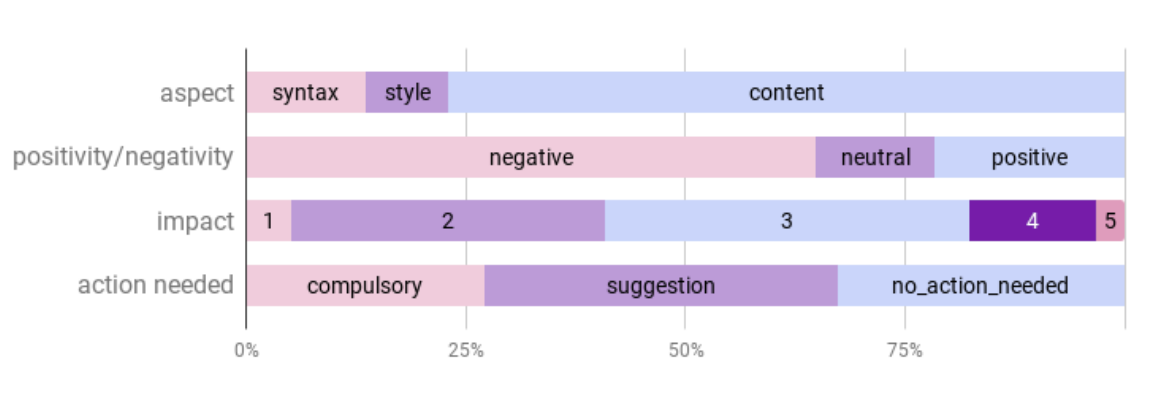
\includegraphics[width=.66\textwidth]{img/nano_annotations}
      \caption[The results of the model expert annotations]{The results of the model expert annotations \cite{nano_peer}}\label{img:annotations}
    \end{figure}
They have applied 18 different lexicon-based sentiment analysis tools to compare the results and found that the best performing tool was the SOCAL method \cite{socal} with a maximum accuracy of 72.8~\%. Most of the methods performed quite poorly according to the authors, however they discovered that the methods with more complex rules performed the best, even if the size of their sentiment lexicon was not large. It is important to note in the context of this work that the sentiment analysis was done separately from the aspects purely focusing on the polarity of the comment and they did not develop or used any tools to automatically determine the aspect of the comment.

Another research that is focused on the processes of scientific publishing and more importantly peer reviewing of these publications builds off of the last paper, however this study is focused on creating a unified model for representation of publications and their assessments \textit{``as well as the involved processes, actors, and provenance in general''} \cite[p. 1]{nanopublications} in the format of linked data. Their vision is that to give more context to reviews, by linking them to other data, such as information about the reviewer and about the author of a paper, as well as provide a way to link specific parts of a review to the part of the paper they comment on.

In their study they performed a user study based on a set of 7 competency questions to determine the practicality of the ontology they propose. The respondents were asked to judge the importance of each of these questions on a scale from 1 to 5 (1 meaning \textit{not important at all} and 5 \textit{very important}). One of these questions,  was \textit{``What is the distribution of the review comments with respect to whether
they address the content or the presentation (syntax and style) of the article?''} which was given the average importance score of 3.64, the second highest importance score in their set of questions. This implies  that the focus of this paper might indeed be valuable for the community, as it focuses on an even more fine-grained aspect-based sentiment analysis of the reviews.

\chapter{Chosen methods of aspect-based sentiment analysis}
\label{sec:chosen_methods}
The next few chapters are about the preprocessing of data and implementation of all the necessary steps of the aspect-based sentiment analysis. In this brief chapter the goal is to describe the chosen methods that were used to give the reader an overall idea of how the sentiment analysis system works before each step is explained in more detail.

Instead of using traditional machine learning methods, the more linguistic-based methods were used as machine learning methods are, as was previously mentioned, not well suited for the task of sentiment analysis on the aspect level. Also, not much research was done in terms of aspect based analysis over conference reviews, and the more linguistic-based methods allow a more hands-on exploration of the data in this specific domain.

The sentiment analysis method is a variation of the holistic lexicon-based approach (see section \ref{sec:holistic_approach}), which expects an existing list of aspect expressions as well as a sentiment lexicon. To extract aspect expression, the taxonomy approach is used (as explained in section \ref{sec:taxonomy}), where the aspects at the top of the hierarchy represent the criteria and all the terms at the second level represent aspect expressions belonging to the criteria. The chosen set of criteria is as follows:
\begin{itemize}
\item Relevance -- relevance of the work to the conference
\item Novelty -- covers novelty of the work as well as its significance and impact
\item Technical quality -- the technical quality of the work
\item State of the art -- if proper research was done on the topic 
\item Presentation -- how well written the paper is, grammar
\item Evaluation -- if the evaluation was carried out properly
\end{itemize}

As some criteria were hard to distinguish even for human annotators, novelty is designed to also cover similar criteria such as significance and impact. Novelty and significance (or impact) may not be equivalent in meaning, however they are often related and influence one another (for example in sentences such as \textit{``In my opinion though the paper does not have a scientific contribution but is a guide\ldots.''}) therefore for simplicity they were joined into one criterion.  

 In order to create a sentiment lexicon for the domain of conference reviews, the Na\"ive Bayes classifier (see section \ref{sec:NBC}) is trained and its output is used to get a lexicon of sentiment/opinion words alongside their polarity. 

The holistic lexicon-based approach is also combined with the sentimentr method (described in section \ref{sec:sentimentr}), which is more complex in the handling of sentiment modifiers than the holistic approach by itself. Instead of using the sentimentr implementation by the authors of the method, the algorithm is implemented based on the sentimentr description provided by the thesis' supervisor as a study material which is available in the attachments, as it allows for a better control of the input and output. The only significant deviation from the study guide as well as the original sentimentr implementation is that negation only influences words that come after it in the sentence. Although it is possible for negation to inverse the polarity of a word that precedes it in a sentence (consider the phrase \textit{``I think not.''}) it is much more common for the negation to come first and it was found that this change in the algorithm works better for the analyzed texts. Also the more common negation with the auxiliary ``do'' such as \textit{``I do not think\ldots''} puts more emphasis on the personal opinion of the speaker while \textit{``I think not.''} is more of a generalized statement \cite{do_not}, and recognizing the reviewer's opinion is the more relevant task.

\chapter{Analysed data}
\section{Source of data}
\section{Data preprocessing}
\subsection{Chosen aspects for extraction}
\subsection{Data preprocessing for aspect vocabulary extraction}
\subsection{Data preprocessing for sentiment vocabulary extraction}
\subsection{Interesting findings during the preprocessing phase}
\section{Previous research on conference paper reviews}

\chapter{Implementation of aspect extraction}
In order to create a lexicon of terms that represent the chosen set of criteria, to be used for identifying aspect expressions in the reviews, I have decided to use two main approaches. One is the taxonomy extraction mentioned in \ref{sec:taxonomy} and the second one is extraction of frequent words used by the reviewers for different criteria in a text that is already divided by headers into sections for the respective criterion.
\section{Manually created taxonomy}
As described in section \ref{sec:taxonomy}, in order to perform taxonomy extraction, we need to manually
create a user defined taxonomy. 

The original idea is that the taxonomy is a hierarchical representation where the top level of the hierarchy represents the feature of an object and the following levels represent the aspects of that feature. Because in my case, I do not need to separate the chosen criteria any further I have used this representation to have the main criteria in the top level and only have one level underneath the top level, to specify possible aspect expressions for each criterion, which serves as a seed for future expansion of the taxonomy by including extracted crude features with enough similarity to the these expressions. 

You can see this taxonomy here \ref{lst:json_tax_m}.

\begin{lstlisting}[language=json,firstnumber=1, caption={Manually created taxonomy for aspect extraction},label={lst:json_tax_m},float,floatplacement=H]
{
    'relevance': {
        'appropriateness', relevance'
    },
    'novelty': {
        'originality', 'innovativeness', 'innovation', 
        'novelty of contribution', 'novelty', 'impact', 'significance'
    },
    'technical quality': {
        'scientific quality', 'implementation', 'soundness',
        'technical quality'
    },
    'state of the art': {
        'scholarship', 'references', 'related work', 
        'state of the art'
    },
    'evaluation': {
    	'reproducibility', 'evaluation'
    },
    'presentation': {
    	'clarity', 'quality of writing', 'presentation'
    },
}
\end{lstlisting}
\section{Crude Features extraction}
The next step of taxonomy based extraction is to obtain a set of crude features. The next two subsections describe the extraction algorithms based on Bings method of aspect extraction.

\subsection{Extraction of frequent nouns and noun phrases}
The first method of extracting terms that are likely to represent an aspect is to extract frequent nouns and noun phrases. For that the content of the file is tokenized and each token is assigned a Part-of-Speech (POS) tag. Then, to get the nouns and noun phrases, the extracted tuples (token, pos\_tag) are parsed to determine the multi-token sequences which represent nouns and NNPs. 

For the parsing I've used the RegexpParser from the nltk library, which utilizes a user defined grammar, consisting of labeled regular expression rules, describing the sequence of POS tags we want to assign the label to. The result of the parsing is a tree structure, where each sequence corresponding to the regular expression is labeled accordingly, so this allows us to pick the subtrees labeled by the parser as noun phrases. 

The code snippet which shows the defined grammar for NP extraction can be seen on listing \ref{lst:np_grammar}. 
The grammar uses POS tags, so NN are nouns, IN are prepositions and JJ are adjectives. The first regular expression, labeled NBAR, searches for nouns and adjectives, terminated with nouns, allowing us to discover phrases like ``black box'', where the meaning changes when we consider both of these words separately. The second regular expression, labeled NP, looks for NBAR expressions connected with prepositions such as ``of'', ``in'' etc.. \cite{nltk_np}

\begin{lstlisting}[language=python,caption={Grammar for the extraction of noun phrases.}, label={lst:np_grammar}]
RegexpParser("""
        NBAR:
            {<NN.*|JJ>*<NN.*>} 

        NP:
            {<NBAR>}
            {<NBAR><IN><NBAR>}
        """)
\end{lstlisting}

In order to then extract only the wanted noun phrase sequences, I traverse the tree, and for each subtree, labeled as NP, I lemmatize each token of the sequence, check if its length is at least two characters, but less than 20 characters, and if so, I join the lemmatized tokens into a single string and append it to the list of NPs in the file.

By performing this extraction with each file, I get a list of lists, where each list represents the extracted nouns and noun phrases from one file. To then obtain the ones that are frequent enough across all the reviews, and may therefore represent aspects, I calculate the support of a noun phrase across the reviews. The following equation represents the calculation of the support metric for a word $w_{i}$ where $N_{w_{i}}$ is the number of reviews containing the word $w_{i}$ and $N$ is the total number of reviews:


$$support(w_{i})=\frac{N_{w_{i}}}{N}$$

In order to perform this calculation I transform the data into a matrix, where each row represents one review, each column represents an aspect candidate and the values of an element in row-i and column-j is 1 if the aspect candidate j is present in review i or 0 if it is not. To get the support of an aspect candidate j, I than divide the sum of column-j by the total number of rows. If the support is greater than the minimum support, the aspect candidate is kept, if not, it is discarded. Through various experiment I found that the best value for minimum support is 2 \%, which gives us reasonable candidates for aspect expressions, but does not include too many candidates to make the process of manually confirming them too tedious. It may seem like a very ``minimal'' minimal support, however the number of reviews I had to my disposal to extract frequent noun phrases was fairly small, so a small support was necessary to account for that fact. It should not be too big of an issue though, considering that the aspect candidates are further tested to determine their similarity to the manually created taxonomy, which reduces the number of aspect candidates the user has to go through.

\subsection{Extraction of frequent adjectives}
Although Bing only focuses on nouns and noun phrases, by going through the training data, I have discovered that fairly often, the aspect expression found in the reviews take the form of adjectives. 

Consider the phrase ``The topic addressed by the paper relevant to the conference.''. Here, the adjective \textit{relevant} evidently corresponds to the aspect \textit{relevance}. Because of that, I have decided to extract frequent adjectives from the reviews as well and again calculate the support of each adjective across the reviews with the same technique as I have used with the noun phrase extraction. 
\section{Extraction by review structure}
The data from the 2018 ESWC conference I have obtained had the review text divided into sections where the different sections represented the different criteria. The structure of these reviews can be seen on figure \ref{img:eswc_2018}, where in bold are the structural part of the review format which stays the same across all reviews. 

I have decided to leverage this data to extract frequent words from each one these sections across the reviews. 

The frequent word of each section are included in the new aspect expression taxonomy directly, they do not go through the same process of similarity matching against the manually created taxonomy as the candidates that were chosen purely on their frequency. This is useful because it allows to extract new possible aspect terms that would not match with any of the terms in the taxonomy, which I originally did not think to  include.

Each term frequent enough in an aspect section across all the reviews is included in the taxonomy based on a match between the ESWC set of aspect and my set of metrics. The mapping between the two sets of metrics was done according to table \ref{table:conf}.

The aspect expression candidates created by this method are still evaluated by the user as explained in section \ref{sec:user_val}.
\begin{figure}[htb]
        \centering
        \fbox{\begin{minipage}{0.9\textwidth}

\textbf{Relevance to ESWC: } 

numerical score (score interpretation)

\textbf{Novelty of the Proposed Solution: } 

numerical score (score interpretation)

\textbf{Correctness and Completeness of the Proposed Solution: }

numerical score (score interpretation)

\textbf{Evaluation of the State-of-the-Art: }

numerical score (score interpretation)

\textbf{Demonstration and Discussion of the Properties of the
 Proposed Approach: }
 
numerical score (score interpretation)
 

\textbf{Reproducibility and Generality of the Experimental Study: }

numerical score (score interpretation)

\textbf{Overall score: }

numerical score (score interpretation)

\textbf{Reviewer's confidence: }

numerical score (score interpretation)

\textbf{Open Reviewing Opting Out:  }

numerical score (score interpretation)

\textbf{Overall evaluation (*Resources and In-Use tracks only*, Research reviewers please only put "n/a"): }

numerical score (score interpretation)





\textbf{----------- Relevance to ESWC ----------- }

reviewer's comment

\textbf{----------- Novelty of the Proposed Solution ----------- }

reviewer's comment

\textbf{----------- Correctness and Completeness of the Proposed Solution ----------- }

reviewer's comment

\textbf{----------- Evaluation of the State-of-the-Art -----------}

reviewer's comment

\textbf{----------- Demonstration and Discussion of the Properties of the Proposed Approach ----------- }

reviewer's comment

\textbf{----------- Reproducibility and Generality of the Experimental Study ----------- }

reviewer's comment

\textbf{----------- Overall score -----------}

reviewer's comment

\end{minipage}}
\caption{ESWC 2018 review structure}
\label{img:eswc_2018}
\end{figure}

\section{Similarity matching against the manually created taxonomy}
After we obtain a set of crude features, the next step is to map these features to the user defined taxonomy. As previously described, we need to calculate the similarity of a crude feature to the aspects in the taxonomy. If the feature is similar enough, it is passed to the final step of the taxonomy extraction, which is an interactive revision process. This process is described in more detail in the next section.

For measuring the similarity between two terms, I have decided to use the wordnet tool and its path\_similarity metric which returns a score denoting how similar two word senses are, based on the shortest path that connects the senses in the hypernym hierarchy. The score is in the range 0 to 1 where 1 denotes identity (when word is compared to itself). \cite{nltk_ps}

The main obstacle of using this metric is that it does not work well with adjectives. That is because all nouns are part of one big hierarchy, but that is not the case for other parts of speech such as adjective, adverb etc.. So for example the similarity for the words ``relevance'' and ``relevant'' is zero, even though the words are closely related. Because the extracted crude features may contain adjectives (in the case of noun phrases) or be adjectives themselves (in the case of frequent adjectives extraction), I have decided to implement a workaround by transforming the adjectives to their closest related noun, and perform the similarity measurement on these nouns. If the similarity of these nouns is greater than the similarity threshold, the original (albeit lemmatized) word is passed on. 

Another issue is measuring similarity with terms consisting of multiple words. Certain multi-token terms are already present in the wordnet thesaurus (such as \textit{state of the art}), and getting their synsets to perform similarity matching is as simple as replacing the spaces between words with underscores. However some multi-token words included both in the user defined taxonomy and in the crude features cannot be found in wordnet directly.

To solve this issue I have decided to calculate the maximum similarity between each token of one term to all the tokens of the other term. Of these similarities I then choose the maximal one.

The final pseudocode for similarity measuring between two terms is on figure \ref{img:sim_alg}. When comparing frequent adjectives to the taxonomy, the part-of-speech argument is set accordingly.
\begin{figure}

\begin{algorithm}[H]
\KwData{term 1, term 2, part-of-speech}
\KwResult{the similarity of the term as a numeric score between 0 and 1}
\For{both terms}
   {	
	\If {the term is just one word}
		{
		term\_synsets = find all synsets of the term \;
		\If{the part-of-speech is adjectives}
			{term\_synsets += find all sysets of the closest related noun}
	}

	\Else
		{ 
		term\_underscored = substitute all spaces in the term with underscores \;
		term\_synsets = find all synsets of term\_underscored \;
	}
	\If{no synsets are found for a multi-word term}
		{
		term\_synsets = synsets of all words in the term (including transformed adjectives) \;
		}
}
score = maximum similarity between all term\_synsets of term1 and term\_synsets of term2 \;
\Return{score}

\end{algorithm}
 \caption{Algorithm for similarity measurement between two terms}
	\label{img:sim_alg}
\end{figure}

Another issue of wordnet's path\_similarity is that it is asymmetrical. So sometimes path\_similarity(x,y) returns None or 0 while path\_similarity(y,x) returns a non-zero value. This is because for some words, a fake root in the hierarchy may be added to find a path between to two words, but this depends on the order in which the two words are supplied to the path\_similarity function. 

Therefore the final calculation of similarity between two terms term1 and term2 is defined as the maximum between similarity(term1,term2) and similarity(term2,term1).

The threshold for similarity of a term to the taxonomy was set to 0.3. Therefore every term with a similarity to any term in the manually created taxonomy equal or greater than the threshold will become an aspect expression candidate under the same aspect as the term it was most similar to.
\section{User validation of final taxonomy}
\label{sec:user_val}
When aspect expression candidates are generated and sorted by the aspect they most likely represent they have to pass the final validation. This validation is a manual process, where a user goes through every aspect candidate and decides between three options:
\begin{itemize}
\item The aspect expression candidate is added under the aspect which was algorithmically determined as the most probable.
\item The user disagrees with the most probable aspect aspect and sorts the aspect expression candidate under a different aspect.
\item The user decides not to include the aspect expression candidate in the taxonomy at all.
\end{itemize}

The interactive process of the user validation of the final taxonomy can be seen on figure \ref{img:user_tax}.
\begin{figure}[htbp!]

\begin{commandshell}
Does the term "topic" belong under aspect "relevance" ? [y/n]
@y@
Does the term "relation" belong under aspect "relevance" ? [y/n]
@n@
Does it belong under any of these aspects ?:
relevance                [a]
novelty                  [b]
technical quality        [c]
state of the art         [d]
evaluation               [e]
presentation             [f]

none of the above        [n]
@n@
Does the term "introduction" belong under aspect "novelty" ? [y/n]
@n@
Does it belong under any of these aspects ?:
relevance                [a]
novelty                  [b]
technical quality        [c]
state of the art         [d]
evaluation               [e]
presentation             [f]

none of the above        [n]
@p@
\end{commandshell}
\caption{The interactive process of user validation of proposed aspect taxonomy.}
\label{img:user_tax}
\end{figure}
\section{Resulting taxonomy of aspects}

\chapter{Creation of sentiment lexicon}
Through some initial experimentation with various existing sentiment lexicons such as the SenticNet sentiment lexicon and the NLTK's SentiWordNet sentiment lexicon it was discovered that these universal sentiment lexicons are not well suited for application on the domain of conference paper reviews.

One issue is that both of these sentiment lexicons assign sentiment polarity on a scale. Therefore most dictionary words have a certain sentiment polarity which was considered inappropriate in this task, as words which would generally be considered neutral should not somehow skew the polarity of words that might actually be important. These words often have a polarity around the center of the polarity interval (for example if the polarity is assigned on a scale from -1 to 1 they usually have polarity somewhere around 0) and could be removed by using some polarity threshold. However, that might also lead to losing some words that are actually important for sentiment classification in this domain. For example in SenticNet, the word \textit{clarification} has polarity of -0.09, but it is often used in sentences such as \textit{``The section about experimental results needs some clarification''} where the sentiment is clearly negative.

Another possible issue with pre-made sentiment lexicons is that they mostly do not include punctuation. However, punctuation might have great semantic significance in conference paper reviews, as they are often written in plaintext and punctuation is used to compensate for the lack of usual formatting styles such as bullet points. 


For that reason, it was decided to create a custom, domain-specific sentiment lexicon. This chapter describes the process of compiling a sentiment lexicon from a set of annotated sentences taken from reviews using the Na\"ive Bayes classifier.
\section{Implementation of sentiment lexicon generation using Naive Bayes}
The Na\"ive Bayes classifier, as described in section \ref{sec:NBC} is a probabilistic classifier which needs a training dataset of labeled data in order to determine the influence of different evidence on the class. The obtainment of this dataset is described in section \ref{sec:data_sl}.

NLTK's implementation of the classifier was used. Of all the lemmatized tokens in the reviews, the number of tokens the classifier needs to process was limited to 450. The tokens are considered features by the algorithm, each token being transformed into a column where the value of the column for each row representing a review is true or false depending on the presence of the token in the review. This was achieved thanks to the \texttt{FreqDist} class from the NLTK's \texttt{probability} module.

The dataset of labeled review sentences was split to have a testing dataset of 50 example sentences to determine the accuracy of the classifier and the rest of sentences was used for training. The test dataset is fairly small, but it was considered far more preferable to leave most examples to the training dataset to produce a hopefully more accurate sentiment lexicon, even though the trade-off is not being able to judge the created lexicon in great detail in this phase. 
That being said, the accuracy of the classifier on the testing dataset was 0.78, meaning 78~\% of sentences were classified correctly. 

The classifier allows us to get a list of features which have the highest contribution to classification through its \texttt{show\_most\_informative\_features} method which based on the number we specify as its argument outputs a list of features with their ratio of occurrences in negative and positive sentences. The output when applied to the training data can be seen in Table \ref{tab:nbc_output}. It shows that it is more than 35 times more likely that the word \textit{easy} occurs in a sentence labeled as \textit{positive} while a question mark occurs far more often in negative sentences.

\begin{table}[htbp!]
\caption{Output of the Na\"ive Bayes classifier}\label{tab:nbc_output}
\centering
\begin{tabular}{lll}
\textbf{Most Informative Features} & \textbf{}         & \textbf{}  \\
easy = True                        & positi : negati = & 35.8 : 1.0 \\
interesting = True                 & positi : negati = & 15.3 : 1.0 \\
but = True                         & negati : positi = & 14.8 : 1.0 \\
topic = True                       & positi : negati = & 13.7 : 1.0 \\
? = True                           & negati : positi = & 12.3 : 1.0 \\
what = True                        & negati : positi = & 10.9 : 1.0 \\
sound = True                       & positi : negati = & 10.6 : 1.0 \\
community = True                   & positi : negati = & 9.9 : 1.0  \\
not = True                         & negati : positi = & 8.9 : 1.0  \\
idea = True                        & positi : negati = & 8.1 : 1.0  \\
interest = True                    & positi : negati = & 7.9 : 1.0  \\
good = True                        & positi : negati = & 7.5 : 1.0  \\
clearly = True                     & positi : negati = & 7.4 : 1.0  \\
well = True                        & positi : negati = & 7.4 : 1.0  \\
me = True                          & negati : positi = & 7.2 : 1.0  \\
bring = True                       & positi : negati = & 6.8 : 1.0  \\
valuable = True                    & positi : negati = & 6.4 : 1.0  \\
why = True                         & negati : positi = & 5.6 : 1.0  \\
conference = True                  & positi : negati = & 5.6 : 1.0  \\
write = True                       & positi : negati = & 5.5 : 1.0  \\
effort = True                      & positi : negati = & 5.4 : 1.0  \\
highly = True                      & positi : negati = & 5.2 : 1.0 
\end{tabular}
\end{table}
The \texttt{show\_most\_informative\_features} method was then adjusted to create a function which transforms these ratios of occurrences in sentences with positive or negative sentiments into a sentiment lexicon. 

Each of the most informative tokens is given a value of -1 or +1 depending on if they occur more often in negative or positive sentences (where -1 corresponds to negative sentiment and  +1 corresponds to positive sentiment). 

\section{Created sentiment lexicon}
From the list of most informative features, the top 100 words were chosen to be included to the sentiment lexicon (setting the ratio threshold at 2.4 : 1.0). 
Then the results were compared with the SenticNet sentiment lexicon, to see what is the level of agreement between the two lexicons and it was discovered that in 13 cases, the polarity of the sentiment of words found in both lexicons differed and in 31 cases a word from my lexicon was not found in SenticNet. Surprisingly not all the words that were not found in SenticNet were not found due to the aforementioned lack of punctuation in SenticNet or because these words could truly be considered neutral. SenticNet was missing some words which are considered fairly meaningful in sentiment analysis such as \textit{rather} or \textit{should}.

A list of 40 positive and 66 negative words compiled manually during the process of labeling the training dataset was also included. The resulting sentiment lexicon contains 186 sentiment words out of which 88 have positive polarity of +1 and 98 have a negative polarity of -1.




\chapter{Implementation of aspect-based sentiment analysis for conference paper reviews}
\section{Design of classes}

 \subsection{Review}
 \begin{figure}[H]
\centering
\begin{tikzpicture}
  \begin{class}[text width=8cm]{Review}{0,0}
    \attribute{file\_name : string}
	\attribute{sentences : list}
	\attribute{criteria : dictionary}
    \operation{get\_scores() : dictionary}
    \operation{add\_score(criterion : string, value: int)}
    \operation{print\_results()}
  \end{class}
 
\end{tikzpicture}

\caption{Review class diagram}
\label{img:review}
\end{figure}

Each review is represented by the \texttt{Review} class. When the class is initiated with its constructor the attribute \texttt{file\_name} is initialized with the file\_name of the review (for the purpose of printing the results). The review text is the tokenized into sentence using NLTK's \texttt{sent\_tokenize} function. To keep track of the numerical scores of the review, which are assigned through the process of sentiment analysis, there is a dictionary \texttt{criteria}, in which the keys of the dictionary are the set of generic criteria as chosen in section INSERT. The values are represented by the \texttt{CriterionScore} class described in section INSERT.

The class has also three methods. The \texttt{add\_score} method accepts the name of a criterion and a sentiment value (-1 or +1) that should be added to the criterion and updates the \texttt{criteria} dictionary accordingly. The \texttt{get\_scores} function returns the final scores for a review in the form of a dictionary where the different criteria are the keys and the values are the numerical scores normalized between 1 and 5. Finally the \texttt{print\_results} function outputs the scores of the review onto the command line in a format shown on figure \ref{img:r_results}.
\begin{figure}[!htb]
\centering
\begin{tabular}{c}
\begin{lstlisting}
row233.txt
	relevance                       3
	novelty                         5
	technical quality               1
	state of the art                5
	evaluation                      2
	presentation                    1
\end{lstlisting}
\end{tabular}
\caption{Example output of the \texttt{print\_results} method of the \texttt{Review} class}
\label{img:r_results}
\end{figure}

\subsection{Sentence}
\begin{figure}[H]
\centering
\begin{tikzpicture}
\begin{class}[text width=8cm]{Sentence}{0,0}
    \attribute{tokens : list}
    \attribute{sentence : string}
    \attribute{sentence\_original : string}
    \attribute{aspects : list}
    \attribute{opinion\_words : list}
    \attribute{criterion\_orientation : dictionary }
	\attribute{unoriented\_aspects : list }

    \operation{print\_results()}
  \end{class}
\end{tikzpicture}
\caption{Sentence class diagram}
\label{img:sentence}
\end{figure}

The \texttt{Sentence} class represents one sentence from a review. When initialized the original sentence is kept in the \texttt{sentence\_original} attribute for printing purposes, however for the needs of the sentiment analysis the sentence is also tokenized and lemmatized. I have used the \texttt{MWEtokenizer} here as well as NLTK's \texttt{word\_tokenize} function. The \texttt{MWEtokenizer} takes a string in the form of a list of tokens and
retokenizes it, ``merging multi-word expressions into single tokens, using a lexicon of MWEs'' INSERT. The reason is that because some aspect expression are multi-words expressions, such as ``state of the art'' I need to keep them as single tokens, in order for them to be recognized when matching the sentence against the aspect taxonomy. Therefore each aspect in the taxonomy is added as a multi-word expression to the \texttt{MWEtokenizer} lexicon. 

The tokens are also lemmatized, with the exception of adjective to keep words such as ``better'' to be lemmatized to ``good'' (the reasoning behind that was explained in section INSERT).
The tokenized and lemmatized sentence is then kept in the \texttt{tokens} attribute of the class and the lemmatized tokens are stringed back together in the \texttt{sentence} attribute. 

For the sentiment analysis algorithm it is also key to know which aspect expressions and which sentiment words the sentence contains. To get a list of aspect expressions I call the \texttt{Taxonomy}'s class method \texttt{get\_aspects}, which compares the tokens it gets as an argument with the taxonomy of aspects and returns the matches as a list of the \texttt{Aspect} class objects. The list of aspect expression is kept in the \texttt{aspects} attribute of the class.

To get a list of sentiment words the \texttt{find\_opinion\_words\_sentiment} function is called, which belongs to the sentimentr module. This function gets a list of tokens as an argument and then for each token that is found in the sentiment lexicon it calculates the polarity value using the sentimentr method (described in section INSERT). It returns a list of (sentiment word, polarity) tuples, which are then used to initialize the \texttt{OpinionWord} class. However if there is an overlap between a sentiment word and an aspect expression, the word is at this point discarded (it may be used in the future, if the orientation of an aspect expression is not found any other way as explained in more detail in section INSERT). The list of sentiment expression is kept in the \texttt{opinion\_words} attribute.

If the main part of the sentiment analysis algorithm fails for an aspect expression (it evaluates the polarity at zero) there is a set of rules which try to determine the sentiment in some other ways. The list of aspect expressions which need the further evaluation is kept in the \texttt{unoriented\_aspects} attribute to which these aspects are continuously added as the review is analyzed.

To keep a track of which criteria a sentence is focused on as well as the polarity of the opinion that is expressed, there is the \texttt{criterion\_orientation} attribute, which is a dictionary where the keys are the criteria and the values are numerical scores.

The \texttt{Sentence} class contains a single method, \texttt{print\_results}, which allows the user to see the results of the analysis on a more fine-grained level than the \texttt{print\_results} method of the \texttt{Review} class. It prints the original sentence and for each criterion in the sentence shows if the polarity of the opinion on the criterion is positive, negative or neutral.


\subsection{OpinionWord}
\begin{figure}[H]
\centering
\begin{tikzpicture}
\begin{class}[text width=8cm]{OpinionWord}{0,0}
    \attribute{name : string}
    \attribute{sentiment\_score : float}
  \end{class}
\end{tikzpicture}
\caption{OpinionWord class diagram}
\label{img:opinionword}
\end{figure}

The \texttt{OpinionWord} class represent an opinion/sentiment word with the name of the word in the \texttt{name} string attribute and the sentiment polarity determined by the sentimentr algorithm kept in the \texttt{sentiment\_score} attribute as a decimal value.

\subsection{CriterionScore}
\begin{figure}[H]
\centering
\begin{tikzpicture}
\begin{class}[text width=8cm]{CriterionScore}{0,0}
    \attribute{criterion : string}
    \attribute{score : int}
    \attribute{count : int}
  \end{class}
\end{tikzpicture}
\caption{CriterionScore class diagram}
\label{img:criterionscore}
\end{figure}

The \texttt{CriterionScore} class is to keep track of the six main criteria which the reviews are evaluated by. The \texttt{criterion} string attribute is assigned the name of the criterion, the \texttt{score} attribute keeps track of the numerical score of the criterion and the \texttt{count} attribute counts the number of times new value is added to the \texttt{score}. Any time an aspect expression belonging to the criterion is discovered in a sentence and its orientation is evaluated by the sentiment analysis algorithm it is added to the \texttt{score} attribute so the \texttt{count} attribute allows as to count the average value so all scores are normalized.

\subsection{Taxonomy}
\begin{figure}[H]
\centering
\begin{tikzpicture}
\begin{class}[text width=8cm]{Taxonomy}{0,0}
    \attribute{aspects : dictionary}
    \attribute{aspect\_names : list}
    \attribute{criteria : list}
    
    \operation{get\_aspects(tokens : list) : list}
    \operation{aspect\_words\_overlap(word : string) : bool}
    
  \end{class}
\end{tikzpicture}
\caption{Taxonomy class diagram}
\label{img:taxonomyclass}
\end{figure}

The \texttt{Taxonomy} class represents the taxonomy created in INSERT. The class is initiated only once, when the taxonomy is loaded from the JSON file in which it was saved during the taxonomy generation phase. The \texttt{aspects} attribute is a python dictionary which follows the same structure as the JSON (see figure INSERT).  For simplicity of other operation the \texttt{criteria} attributes keeps a list of all the main criteria/metrics, while the \texttt{aspect\_names} attribute keeps track of all aspect expressions in the taxonomy.

There are two method in the class, the method \texttt{get\_aspects} accepts a list of tokens in a sentence, finds if any of the tokens are aspect expressions and if so, returns a list of the \texttt{Aspect} class objects that correspond to them. The second method \texttt{aspect\_words\_overlap} accepts a string as an argument and returns \textit{True} if the string overlaps with a string of an aspect expression and \textit{False} otherwise.


\subsection{Aspect}
\begin{figure}[H]
\centering
\begin{tikzpicture}
\begin{class}[text width=8cm]{Taxonomy}{0,0}
    \attribute{criterion : string}
    \attribute{name : string}
    \attribute{adjective : bool}
  \end{class}
\end{tikzpicture}
\caption{Aspect class diagram}
\label{img:aspectclass}
\end{figure}

The \texttt{Aspect} class simply represents an aspect expression, the name of which is saved in the \texttt{name} attribute. It also keeps the name of the criterion/metric under which the aspect expression belongs in the \texttt{criterion} attribute, in the form of a string. 

If the aspect is an adjective the \texttt{adjective} attribute is set to \textit{True} to enable some special handling of these expressions. The value of \texttt{adjective} is determined by finding the wordnet synsets of the expression and if the POS tag of any of the synsets is that of an adjective (in NLTK's wordnet implementation that means the tag is either \textit{a} for an adjective or \textit{s} for satellite adjectives).

\section{Description of the algorithm}
\begin{figure}[htbp!]
\begin{algorithm}[H]
% Set Function Names
  \SetKwFunction{FMain}{opinion\_orientation}



  \SetKwProg{Fn}{Function}{:}{\KwRet}
  \Fn{\FMain}{
       \For{each sentence $s_{i}$ that contains a set of aspect expressions}    
        { 
        	\If{the number of aspect expressions in $s_{i}$ > 5}
    			{
      				continue\;
    			}
    		\For{each aspect $a_{j}$ in $s_{i}$}
    		{
    			$orienation$ = 0\;
    			\For{each opinion word $ow_{k}$ in $s_{i}$}
    			{
    				$distance$ = \textbf{distance\_betweeen\_words}($ow_{k}$, $a_{j}$, $s_{i}$)\;
    				$orientation$ += $\frac{ow_{k}.sentiment\_score}{distance}$\;
    				
    			}
    			
    			\eIf{$orientation$ > 0}
    		{ 
    			$orientation$ = 1\;
    		}
    		{
    		\eIf{$orientation$ < 0}
    		{
    		$orientation$ = -1\;
    		}
    		{
    		$orientation$ = 0\;
    		}
    		}
    			\eIf{$orientation$ = 0 and $a_{j}$ is an adjective}
    		{
				$orientation$ = 1\;   
    		}
    		
    		{
    			add $a_{j}$ to $s_{i}$'s unoriented\_aspects\;
    		}
    			$a_{j}$'s criterion orientation in $s_{i}$ += $orientation$\;
    			\textbf{review.add\_score}($a_{j}$'s criterion, orientation)
    		}
    		\For{aspect $a_{l}$ in $s_{i}$'s unoriented aspects}
    		{
    		$orientation$ = \textbf{apply\_intra\_sentence\_rules}($s_{i}$, $a_{l}$)\;
    		\If{$orientation$ = 0}
    		{
    			$sentiment$ = \textbf{find\_opinion\_words\_sentiment}($a_{l}$)\;
    		}
    		
    		
    		\eIf{$orientation$ > 0}
    		{ 
    			$orientation$ = 1\;
    		}
    		{
    		\eIf{$orientation$ < 0}
    		{
    		$orientation$ = -1\;
    		}
    		{
    		$orientation$ = 0\;
    		}
    		}
    		$a_{l}$'s criterion orientation in $s_{i}$ += $orientation$\;
    		\textbf{review.add\_score}($a_{l}$'s criterion, orientation)
    		}
    		}
  }
\end{algorithm}
\caption{opinion\_orientation algorithm}
\label{img:opinion_orientation}
\end{figure}

%%%%%%%%%%%%%%%%%%%%%%%%%%%%%%%%%%%%%%%%%%%%
\begin{figure}[h]
\begin{algorithm}[H]
% Set Function Names
  \SetKwFunction{ISR}{apply\_intra\_sentence\_rules}



  \SetKwProg{Fn}{Function}{:}{\KwRet}
  \Fn{\ISR}{
	\For{each opinion word $ow_{i}$ in the sentence}
	{
		$words\_between$ = words between $aspect$ and $ow_{i}$\;
		\If{adversative in $words\_between$}
		{
			\Return{$-1\times ow_{i}.sentiment\_score$}
		}
	}
}
\end{algorithm}
\caption{apply\_intra\_sentence\_rules algorithm}
\label{img:intra_sentence}
\end{figure}

%%%%%%%%%%%%%%%%%%%%%%%%%%%%%%%%%%%%%%%%%%%


The aspect-based sentiment algorithm that I have created for the task of extracting criteria orientations from a text is loosely based on the algorithm mentioned in section INSERT, but I have made some changes. The main part of the algorithm is shown on figure \ref{img:opinion_orientation}. 

\subsection{Determining opinion orientation using aspect expressions and sentiment words in a sentence}

For each review we iterate through its sentences (which are here objects of class \texttt{Sentence}). If the number of aspect expressions in the sentence is more than 5 the sentence is not evaluated. That is because if the number of aspects is that high in a single sentence it would be hard to evaluate which opinion words belong to which aspect. It is especially an issue with the numerical evaluations at the beginning of reviews, which are sometimes not structured by newlines or any other separator.

Given a sentence $s_{i}$ that contains a set of aspect expression we compute a sentiment polarity score for the expression. Given a set of sentiment words in the sentence, we calculate their influence based on the sentiment score given by the sentimentr algorithm which is divided by the distance of the sentiment word from the aspect expression. These scores are then aggregated by a sum function for each aspect expression.

An expression is assigned the sentiment polarity of +1 if it is positive and -1 if it is negative, 0 if the polarity was not determined. If the polarity is 0, it is added to the list of unoriented aspects of a sentence for further processing, but if we succeeded in determining the polarity, the score for an criterion under which the aspect expression belongs in the taxonomy is adjusted in the review as well as the sentence.
\subsection{Adjectives as aspect expressions}
When for some aspect expressions the orientation is unknown after aggregating polarities of nearby opinion words they are added to $s_{i}$'s list of unoriented aspects. These aspect expressions are then first evaluated using the adjective rule, where if the aspect expression is an adjective, it may be used as an opinion word itself. That is the case in sentences such as ``This paper is highly relevant to the conference'', where the adjective \textit{relevant} points to the relevance criterion, but also expresses a positive polarity on said criterion. 

In cases when the aspect expression is an adjective, its polarity is determined using the sentimentr algorithm as if it was an opinion word, to cover cases such as negation.

\subsection{Intra sentence rules}
If the aspect expression orientation is still unknown after the use of the adjective rule it is evaluated using the intra sentence rules, which rely on the fact that a sentence only expresses one polarity unless it includes an adversative conjunction.

For each so far unoriented aspect expression we find the closest opinion word and all the words between the aspect and the opinion word. If there is a adversative conjunction in between the opinion word and the aspect expression, that likely means the sentiment polarity was inverted by the conjunction and therefore the aspect expression should be given the opposite polarity of the opinion word. This should help in sentences such as ``The evaluation shows great results but the dataset was small.'' in which \textit{dataset} might be an aspect expression pointing to the evaluation criterion but \textit{small} might not be in the sentiment lexicon (for a human, it is easy to point to small as a negative word here based on the context, but that is not always the case, like in a phrase \textit{small error} it would be positive). The closest identified opinion word in this sentence would be \textit{great}, with a positive polarity, but given the fact that there is \textit{but} in between \textit{great} and \textit{dataset}, the polarity assigned would be negated.

If no adversative conjunction is found, the aspect expression is given the polarity of the closest opinion word without any changes, following the \textit{one sentence -- one polarity} idea. 

\subsection{Sentences with neutral sentiment}
If the orientation of an aspect expression is still 0 after the application of all rules, it is finally evaluated as neutral. Sometimes, this might mean that the sentiment was present but expressed in a way that the algorithm did not recognize. It might also mean a false positive for an aspect identified within a sentence. That is because there might be an overlap between aspect expressions and expression that are often used within the field for describing an idea presented in a paper . Take the sentence ``In this paper authors investigate how state-of-the-art language technologies can be ported to the historical ecology domain.'' in which the algorithm would think that the \textit{state-of-the-art} expression points to the state of the art criterion but here it is simply a statement about the objective of the paper. 

These aspect expression do not influence the numerical scores of a review, the aspects with neutral orientation are however still shown in the algorithm's output at a sentence level.

\chapter{Evaluation of results}
\chapter*{Conclusion}
\addcontentsline{toc}{chapter}{Conclusion}
The aim of this thesis was to try to build a system for extracting opinions and sentiment from conference paper reviews. The objective was to determine if there is a way to successfully detect perceived value of a paper, based on sentiment analysis of its reviews.
The results of this work show that the creation of an aspect-based sentiment analysis system focused on the domain of conference paper reviews is indeed possible. 

In the practical part of this thesis a system was implemented, that analyzes a review following these steps: First an identification of which aspect of a paper each sentence of a review is commenting on. This is done by using a dictionary of aspect expressions, where each expression falls under one of the six chosen criteria -- \textit{relevance}, \textit{novelty}, \textit{technical quality}, \textit{state of the art}, \textit{presentation} and \textit{evaluation}. Then it applies a dictionary-based method of sentiment analysis using a custom-built domain specific sentiment lexicon to determine the sentiment polarity of the criterion expression. By grouping the aspect expression polarities by the criteria to which they belong the system outputs numerical scores for each criterion on a scale from 1 to 5. It also lists all sentences of a review in which an aspect expression was identified, stating the respective criterion and its sentiment polarity in the sentence.

To evaluate the precision of such a system the numerical evaluation output of the reviews created by the algorithm was then compared to the original numerical scores from a set of reviews and the results were also evaluated in more detail by calculating the precision and recall of criterion identification on a sentence level. Based on the results of the evaluation a set of recommendations was given for future improvements, one of which being an acquirement of a significantly larger training dataset. Most conferences do not make their reviews publicly available and this was a considerable limitation of the implementation. In this aspect the secondary and unexpected objective of this thesis is to serve as a motivation for an easier accessibility of this kind of data. 

The evaluation of sentiment analysis accuracy shows an improvement on the results of similar existing research and so with indicated improvements the system is going to be a valuable tool for helping to facilitate the meta-reviewing process. It can also help with the unification of criteria scores across different conferences and reviewers using the numerical scores outputted by the system.

All the algorithms created in this work -- the aspect expression identification, sentiment lexicon compiler and aspect-based sentiment analysis -- are implemented in a way which would require slight adjustments for application on a number of different domains of conferences. The main change that would be required is to manually create a new taxonomy of aspect expressions serving as a base for identification of other aspect expressions, helping to define the set of the domain-specific criteria. Allowing for minor adjustments, the practical use of the system in other domains is clear,  providing the appropriate datasets to retrain the algorithm for the new application.

I am currently taking part in a project aimed at creating a generator of pictorial metaphors of reviews to simplify the difficult task of meta-reviewing by mapping the numerical scores of criteria to different parts of an image of a car \cite{pictoreview_iswc}. The developed system has the potential to eventually work as an extension of this tool by allowing its use for reviews where the numerical scores are missing. This is just one of the many examples of future use of the system described in this thesis.

\sloppy
Should the reader of this thesis be inclined to find out more,
the implementation is publicly available at \url{https://github.com/jurs02/aspect-based-sentiment-analysis-of-conference-submission-reviews}.

\fussy





%%% Seznam použité literatury
%% Toto platí v případě použití samostatné bibliografické databáze
\printbibliography[title={References},heading={bibintoc}]

%% Toto platí v případě použití prostředí thebibliography
%% Pro sestavení citačních údajů lze doporučit:
%%     https://knihovna.vse.cz/citace/priklady/
%%     https://www.citace.com/
%\openright
%\phantomsection
%\addcontentsline{toc}{chapter}{\bibname}
%\begin{thebibliography}{99}
%\bibitem{Cermak2018}ČERMÁK, Radim, SMUTNÝ, Zdeněk. A Framework for Cultural Localization of Websites and for Improving Their Commercial Utilization. In:  \emph{Global Observations of the Influence of Culture on Consumer Buying Behavior} [online]. Hershey~: IGI Global, 2018, s. 206--232. ISBN 978-1-5225-2727-5. DOI: 10.4018/978-1-5225-2727-5.
%
%\bibitem{Hladik2018}HLADÍK, Milan, ČERNÝ, Michal. The Shape of the Optimal Value of a Fuzzy Linear Programming Problem. In: \emph{Fuzzy Logic in Intelligent System Design} [online]. Cancum, 16.10.2017 -- 18.10.2017. Cham~: Springer, 2018, s. 281--286. Advances in Intelligent Systems and Computing 648. ISBN 978-3-319-67136-9. DOI: 10.1007/978-3-319-67137-6\_31.
%
%\bibitem{Jasek2018}JAŠEK, Pavel, VRANÁ, Lenka, ŠPERKOVÁ, Lucie, SMUTNÝ, Zdeněk, KOBULSKÝ, Marek. Modeling and Application of Customer Lifetime Value in Online Retail. \emph{Informatics} [online]. 2018, roč. 5, č. 1. 22 s. eISSN 2227-9709. DOI: 10.3390/informatics5010002. Dostupné také z: \url{http://www.mdpi.com/2227-9709/5/1/2/pdf}.
%
%\bibitem{Pecakova2018}PECÁKOVÁ, Iva. \emph{Statistika v terénních průzkumech}. 3. přeprac. vyd. Praha~: Professional Publishing, 2018. 254 s. ISBN 978-80-88260-10-3.
%\end{thebibliography}


%%% Přílohy k bakalářské práci, existují-li. Každá příloha musí být alespoň jednou
%%% odkazována z vlastního textu práce. Přílohy se číslují.
\part*{Attachments}
\appendix
\chapter{}


% \include{...}
% \include{...}

\end{document}
